\section{Celda Sedra-Ghorab-Martin}

\subsection{Introducci\'on}
En este apartado se realiza un an\'alisis de la celda denominada Sedra-Ghorab-Martin, y posteriormente el dise\~no, s\'intesis y an\'alisis de un filtro activo empleando dicha celda. La principal fuente de informaci\'on ser\'a el paper denominado \textit{Optimum configurations for Single-Amplifier Biquadratic Filters}

\subsection{La celda Sedra-Ghorab-Martin}

La celda Sedra-Ghorab-Martin (en adelante, \textit{celda SGB}) es un circuito creado en el a\~no 1980 por los miembros de IEEE cuyos nombres se reflejan en el nombre de la celda. Dicho circuito se basa en el circuito pasabanda de Deliyannis, que se reproduce a continuaci\'on.

\begin{figure}[H] \label{fig:EJ3_deliyannis}
    \centering
    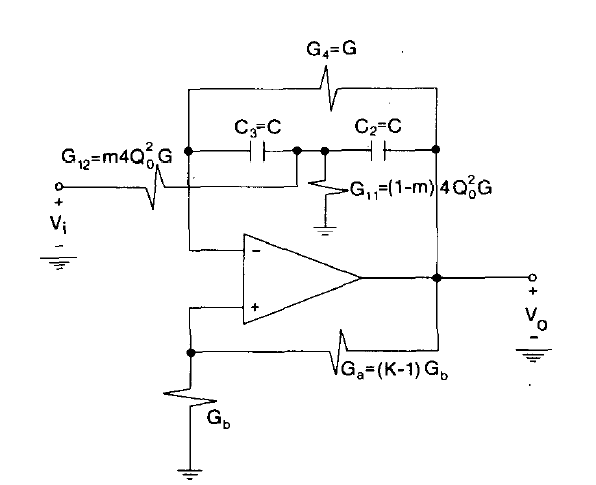
\includegraphics[width=0.8\textwidth]{../EJ3/Resources/deliyannis_cell.png}
    \caption{Pasabanda Deliyannis}
\end{figure}

Donde $k$ es una constante que es directamente proporcional a la cantidad de realimentaci\'on positiva del circuito.

Este circuito es posteriormente generalizado por Friend para poder construir cualquier tipo de configuraci\'on de filtro. El mismo se caracteriza por poseer una alta selectividad, empleando tanto realimentaci\'on positiva como negativa. Sin embargo, para poder sintetizar cualquier tipo de filtro es necesario cargar la red RC que se observa en la realimientaci\'on negativa del circuito~\ref{fig:EJ3_deliyannis}, lo que hace poco realizable el dise\~no del mismo.\\


Por otro lado, se encontr\'o que realizando una transformaci\'on complementaria sobre el circuito de Deliyannis (esto es, intercambiando la salida del amplificador operacional por masa, y procediendo an\'alogamente con la entrada inversora y no inversora del mismo) se deriva en el circuito de Sallen-Key manteniendo una realimentaci\'on positiva. Cabe destacar que esta transformaci\'on conserva la sensibilidad de los polos del circuito, pero no as\'i con los ceros de transmisi\'on del mismo. A\'un asi, se lleg\'o a la conclusi\'on de que es m\'as ventajoso implementar las configuraciones de filtros en una celda Sallen-Key con realimentaci\'on positiva (exceptuando el caso de un filtro pasabanda).\\


En la figura de abajo se observa como aplicando transformaci\'on complementaria y cambios en la red RC se llega a distintos circuitos con la caracter\'istica de poseer una red de realimentaci\'on similares a un circuito Sallen-Key.

\begin{figure}[H] \label{fig:EJ3_transformation_circuits}
    \centering
    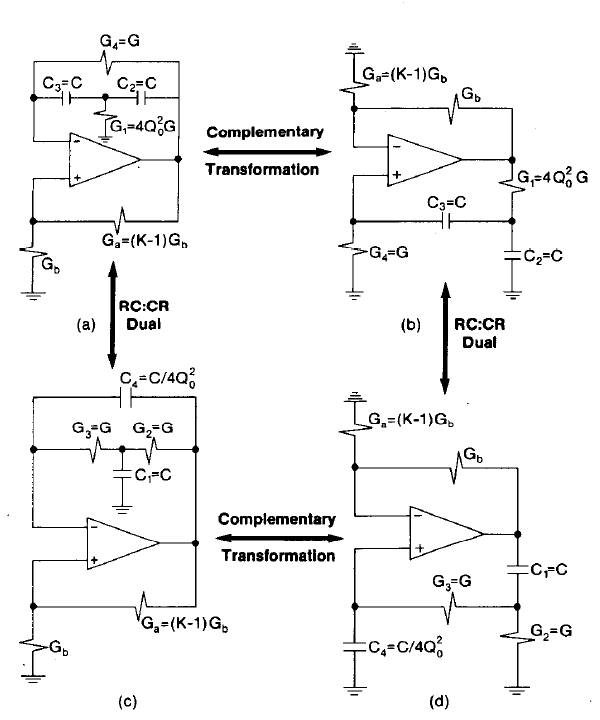
\includegraphics[width=0.7\textwidth]{../EJ3/Resources/transformation_circuits.png}
    \caption{Resultados de las transformaciones}
\end{figure}

Los circuitos \ref{fig:EJ3_transformation_circuits} b) y \ref{fig:EJ3_transformation_circuits} d) son llamados EPF (Enhanced positive feedback), y son la base de la celda SGB. Esta caracter\'istica esta dada por un coeficiente $K>1$. Para los cuatro circuitos de la figura se cumplen las siguientes ecuaciones que describen el comportamiento de los mismos.

\begin{equation}\label{EJ3eq1}
\frac{C}{G} = \frac{2Q_0}{\omega_0}
\end{equation}

\begin{equation}\label{EJ3eq2}
K-1 = \frac{1}{2Q_0^2}\cdot \left( 1-\frac{Q_0}{Q} \right)
\end{equation}

Donde $Q_0$ es un par\'ametro de dise\~no que cumple $Q>Q_0$. De esta forma, los circuitos del tipo EPF permiten implementar filtros con la siguiente funci\'on transferencia de segundo orden

\begin{equation}
\label{transf}
H(s)=\frac{n_2s^2+n_1s+n_0}{s^2+s\left(\frac{\omega_0}{Q}\right)+\omega_0^2}
\end{equation}

Donde los coeficientes $n_i$ determinan los ceros de transmisi\'on, y por ende el tipo de filtro implementado por el circuito. Para poder lograr esto sin afectar la ubicacion de los polos se necesita que aquellos componentes que se encuentren conectados a masa sean desconectados de la misma, total o parcialmente (dividi\'endolos). Asi, se obtienen los dos circuitos HPB (\textit{high-pass biquad}) y LPB (\textit{low-pass biquad})que se muestran en las figuras \ref{EJ3_HPB} y \ref{EJ3_LPB} respectivamente.

\begin{figure}[H]
    \centering
    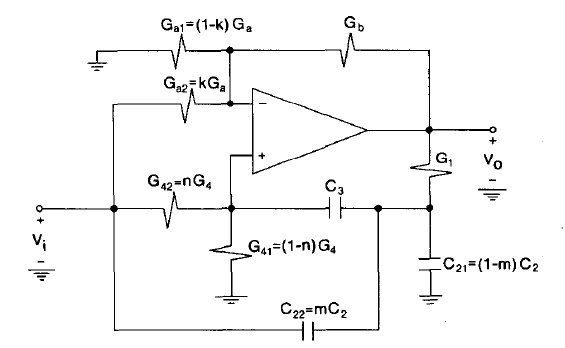
\includegraphics[width=0.7\textwidth]{../EJ3/Resources/HPB.png}
    \caption{High-pass biquad}
     \label{EJ3_HPB}
\end{figure}

\begin{figure}[H] 
    \centering
    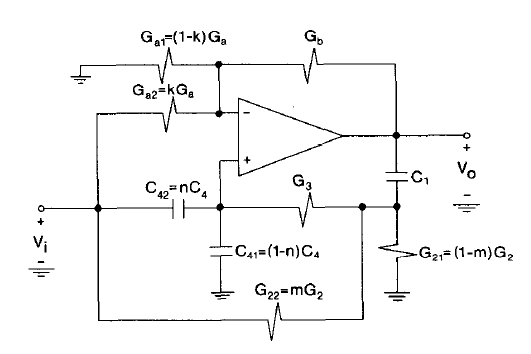
\includegraphics[width=0.7\textwidth]{../EJ3/Resources/LPB.png}
    \caption{Low-pass biquad}
    \label{EJ3_LPB}
\end{figure}

Como sus nombres lo indican, ambos circuitos son empleados para la implementaci\'on de distintos tipos de filtros. El circuito a elegir en funci\'on de la aplicaci\'on elegida se muestra en la tabla a continuaci\'on.

\begin{table}[H]
    \centering
    \begin{tabular}{c c}
        Tipo de Filtro & Circuito Recomendado \\
        \hline
        Pasabajos & LPB (fig.~\ref{EJ3_LPB}) \\
        Pasaaltos & HPB (fig.~\ref{EJ3_HPB}) \\
        Pasabanda & Deliyannis (fig.~\ref{fig:EJ3_deliyannis}) \\
        Pasatodo & LPB o HPB \\
        High pass notch & HPB \\
        Low pass notch & LPB\\
    \end{tabular}
    \caption{Circuitos recomendados}
    \label{tabla_circuitos}
\end{table}

\subsubsection{Ecuaciones de dise\~no}

En la ecuaci\'on~\ref{transf} se muestra la funci\'on transferencia de la celda a implementar. El valor de los coedicientes $n_i$ de la misma est\'an determinados en forma distinta dependiendo del circuito elegido. Para un circuito HPB est\'an descriptos por las siguientes equivalencias.

\begin{equation}
\label{hpbn0}
n_0 = \frac{G_1 \left( G_{41} + G_{42} \right)}{C_3 \left( C_{21} + C_{22} \right)} \cdot \left( \frac{G_{42}}{G_{41} + G_{42}} \cdot \frac{G_{a1} + G_{a2} + G_b}{G_b} - \frac{G_{a2}}{G_b} \right)
\end{equation}

\begin{equation}
\label{hpbn1}
n_1 = \frac{G_{a1} + G_{a2} + G_b}{G_b} \cdot G_{42} \cdot \left( \frac{1}{C_{21}+C_{22}} + \frac{1}{C_3} \right) - \frac{G_{a2}}{G_b} \cdot \left[ \frac{G_1}{C_{21}+C_{22}} + \left( G_{41} + G_{42} \right) \left(  \frac{1}{C_{21}+C_{22}} + \frac{1}{C_3} \right) \right]
\end{equation}

\begin{equation}
\label{hpbn2}
n_ 2 = \frac{G_{a1} + G_{a2} + G_b}{G_b} \cdot \frac{C_{22}}{C_{21}+C_{22}} - \frac{G_{a2}}{G_b}
\end{equation}

Asimismo, se consideran las siguientes dos ecuaciones relativas a par\'ametros caracter\'isticos del denominador de la transferencia del circuito.

\begin{equation}
\label{hpbw0}
\omega_0^2 = \frac{G_1 \left( G_{41} + G_{42} \right)}{C_3 \left( C_{21} + C_{22} \right)}
\end{equation}

\begin{equation}
\label{hpbwoQ}
\frac{\omega_0}{Q} = \left( G_{41} + G_{42} \right) \left(  \frac{1}{C_{21}+C_{22}} + \frac{1}{C_3} \right) - \frac{G_1}{C_{21}+C_{22}} \cdot \frac{G_{a1} + G_{a2}}{G_b}
\end{equation}

An\'alogamente, para un circuito LPB las ecuaciones que caracterizan a la funci\'on transferencia son las siguientes.

\begin{equation}
\label{lpbn0}
n_0 = \frac{G_3 \left( G_{21} + G_{22} \right)}{C_1 \left( C_{41} + C_{42} \right)} \cdot \left( \frac{G_{22}}{G_{21} + G_{22}} \cdot \frac{G_{a1} + G_{a2} + G_b}{G_b} - \frac{G_{a2}}{G_b} \right)
\end{equation}

\begin{equation}
\label{lpbn1}
n_1 = \frac{G_{a1} + G_{a2} + G_b}{G_b} \cdot G_{42} \cdot \left( \frac{C_{42}}{C_{41}+C_{42}} \right) \cdot\ \left( \frac{G_{21}+G_{22}+G_{3}}{C1} \right) - \frac{G_{a2}}{G_b} \cdot \left( \frac{G_3}{C_{41}+C_{42}} + \frac{G_{21}+G_{22}+G_3}{C_1}\right)
\end{equation}

\begin{equation}
\label{lpbn2}
n_ 2 = \frac{G_{a1} + G_{a2} + G_b}{G_b} \cdot \frac{C_{22}}{C_{1}+C_{2}} - \frac{G_{a2}}{G_b}
\end{equation}

\begin{equation}
\label{lpbw0}
\omega_0^2 = \frac{G_3 \left( G_{21} + G_{22} \right)}{C_1 \left( C_{41} + C_{42} \right)}
\end{equation}

\begin{equation}
\label{lpbwoQ}
\frac{\omega_0}{Q} = \left( \frac{G_{21}+G_{22}+G_3}{C_1} \right) - \left( \frac{G_3}{C_{41}+C_{42}} \right) \cdot \left( \frac{G_{a1} + G{a2}}{G_b} \right)
\end{equation}


\subsubsection{Sensibilidades}
Las sensiibilidades del circuito respecto a sus componentes es esencial a la hora de establecer criterios de dise\~no en torno a la celda SGM. A grandes rasgos, se pueden evidenciar dos tipos de sensibilidades: aquellas que corresponden a componentes pasivos (tales como resistores y capacitores), y aquellas relacionadas con dispositivos activos (el amplificador operacional). En este punto juega un papel importante el par\'ametro de dise\~no $Q_0$ antes mencionado. Su valor determina el balance entre los dos tipos de sensibilidades, por lo que su elecci\'on debe ser llevada a cabo considerando los valores de dispersi\'on de ambos grupos de componentes. De esta forma, $Q_0$ se calcula de acuerdo a la siguiente ecuaci\'on.

\begin{equation}
\label{q0}
Q_0 = \left[ |A(s_0)|^2 \cdot \frac{8\sigma_R^2 + \sigma_C^2}{8\sigma_A^2}\right]^{\frac{1}{4}}
\end{equation}  

Donde $\sigma_R$, $\sigma_C$ y $\sigma_A$ representan la variaci\'on de resistores, capacitores y la ganancia del op-amp  respectivamente. Por otro lado $A(s_0)$ es la ganancia del amplificador operacional en la frecuencia nominal del polo $s_0$, siendo esta \'ultima:

\begin{equation}
s_0 = -\frac{\omega_0}{2Q} + j\omega_0\sqrt{1-\frac{1}{4Q^2}}
\end{equation}

Es posible expresar las sensibilidades pasivas de los circuitos HPB y LPB en funci\'on de este par\'ametro, regidas por las siguientes relaciones.


\begin{table}[H]
    \centering
    \begin{tabular}{c | c c}
         & $\omega_0$ & Q\\
        \hline
        $R_1$ ($C_1$ LPB) & $-\frac{1}{2}$ & $-\left(\frac{Q}{Q_0} - \frac{1}{2} \right)$ \\
        $C_2$ ($R_2$ LPB) & $-\frac{1}{2}$ & $-\frac{1}{2}\left(\frac{Q}{Q_0} - 1 \right)$ \\
        $C_3$ ($R_3$ LPB) & $-\frac{1}{2}$ & $\frac{1}{2}\left(\frac{Q}{Q_0} - 1 \right)$\\
        $R_4$ ($C_4$ LPB) & $-\frac{1}{2}$ & $\left(\frac{Q}{Q_0} - \frac{1}{2} \right)$ \\
        $R_a$  & $0$ & $-\left(\frac{Q}{Q_0} - 1 \right)$\\
        $R_b$  & $0$ & $\left(\frac{Q}{Q_0} - 1 \right)$\\
    \end{tabular}
    \caption{Sensibilidades pasivas de un HPB}
    \label{tabla_sensibilidades_pasivas}
\end{table}

Respecto de las sensibilidades activas, es importante considerar la frecuencia de ganancia unitaria del amplificador operacional (o $\omega_t$). Las siguientes dos ecuaciones definen las sensibilidades de $\omega_0$ y Q respecto de dicha frecuencia.

\begin{equation}
S_{\omega_t}^{\omega_0} = Q_0 \cdot \left(\frac{\omega_0}{\omega_t}\right)
\end{equation}

\begin{equation}
S_{\omega_t}^{Q} = -Q_0 \cdot \left(\frac{\omega_0}{\omega_t}\right) \left[ 4Q\left(\frac{\omega_0}{\omega_t}\right) - 1\right]
\end{equation}

Los efectos del ancho de banda finito del amplificador operacional pueden ser minimizados si se tienen en cuenta en una etapa previa al dise\~no. De esta forma, se predistorsionan los valores de $\omega_0$ y $Q$ acorde a las siguientes expresiones.

\begin{equation}
\label{omega_predistortion}
\omega_p = \omega_0 \left[ 1+Q_0\left(\frac{\omega_0}{\omega_t}\right)\right]
\end{equation}

\begin{equation}
\label{q_predistortion}
Q_p = Q \left[ 1-2Q_0Q\left(\frac{\omega_0}{\omega_t}\right)\left(\frac{1}{2Q}-\frac{\omega_0}{\omega_t}\right)\right]
\end{equation}

Como se puede observar en este an\'alisis, se debe elegir de forma \'optima el valor de $Q_0$ (con la ecuaci\'on~\ref{q0}) para lograr un dise\~no realizable y estable.


\subsection{Implementaci\'on de filtro}
Realizado el an\'alisis de la celda en cuesti\'on, se pide implementar un filtro pasaaltos activo con la misma, que cumpla con las condiciones fijadas en la tabla~\ref{tabla_filtro}.

\begin{table}[H]
    \centering
    \begin{tabular}{c c c}
        Par\'ametro & Valor indicado & Valor efectivo \\
        \hline
         $f_a$ & $\left( 10+1,1\cdot \frac{N}{2} \right) kHz$  & $10,55 kHz$  \\
         $f_p$ & $2 \cdot f_a $ & $21,1kHz$  \\
         $A_p$ & $2dB$ & $2dB$ \\
         $A_a$ & $40dB$ & $40dB$  \\
         $Z_{in}$ & $>50k\Omega$ & $>50k\Omega$  \\
    \end{tabular}
    \caption{Especificaciones del filtro}
    \label{tabla_filtro}
\end{table}

En este sentido es importante remarcar que se toma un margen de tolerancia del $15\%$ respecto a las atenuaciones l\'imite en banda atenuada y de paso. De esta forma, para el c\'alculo se tomar\'a $A_p = 1,7dB$ y $A_a = 46dB$. 

El primer paso para el dise\~no del mismo es normalizar la plantilla a una de un pasabajos, con frecuencia angular pasante unitaria ($\omega_{pN} = 1$). Una vez hecho esto se procede a aplicar la aproximaci\'on de Cauer sobre dicha plantilla.

\begin{figure}[H] \label{fig:EJ3_highpass_template}
    \centering
    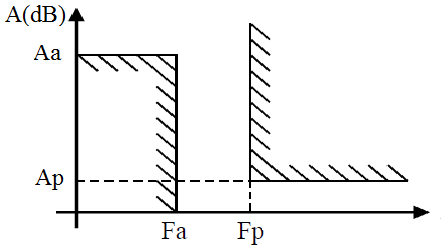
\includegraphics[width=0.5\textwidth]{../EJ3/Resources/highpass_template.png}
    \caption{Plantilla de pasaaltos}
\end{figure}


Cabe destacar que la aproximaci\'on de Cauer es una aproximaci\'on por funciones el\'ipticas, con riple constante tanto en la banda de paso como la de atenuaci\'on. Asimismo, cuenta con el menor error de ponderaci\'on de Chebycheff, por lo que es la aproximaci\'on que tiene la menor banda de transici\'on para un orden dado. Por ende, ser\'a la que, dada una determinada plantilla de filtro, devuelva la funci\'on transferencia de menor orden, de la siguiente forma.

\begin{equation}
|H(j\omega)|^2 = \frac{1}{1+\epsilon_p^2 \cdot F_n^2(\omega)}
\end{equation}

Donde $\epsilon_p$ es el coeficiente de riple en banda de paso y $F_n(\omega)$ es una funci\'on determinada tal que se cumpla la condici\'on de equi-riple en las dos bandas.

Finalmente se desnormaliza la funci\'on transferencia normalizada obtenida para llegar a una que describa un filtro pasaaltos con las caracter\'isticas detalladas anteriormente.

\begin{equation}
H(s) = k \cdot \frac{(s-z_1)(s-z_2)(s-z_3)(s-z_4)}{(s-p_1)(s-p_2)(s-p_3)(s-p_4)}
\end{equation}

Donde $z_1 \approx 7,632 \cdot 10^4 \frac{rad}{s}$, $z_2 \approx 3,428 \frac{rad}{s}$, $z_3 = -z_2$ y $z_4 = -z_1$. Los polos son $p_1 \approx (-1,341\cdot 10^5 +j2,078\cdot 10^5)\frac{rad}{s}$, $p_2 = \overline{p_1}$, $p_3 \approx (-1,258\cdot 10^4 + j1,349\cdot 10^5) \frac{rad}{s}$, $p_4 = \overline{p_3}$. El coeficiente k vale $k \approx 0,8$

En este punto es necesario dividir la funci\'on transferencia del filtro en dos cocientes de polinomios de orden 2, debido a las limitaciones de la celda SGM. De esta forma, se obtienen dos etapas regidas por las siguientes ecuaciones.


\begin{equation} 
\label{transf_stage1}
H_1(s) = \frac{s^2 + 5,825 \cdot 10^9}{s^2 + 2,518 \cdot 10^4 s + 2,191 \cdot 10^7}
\end{equation}

\begin{figure}[H] 
    \centering
    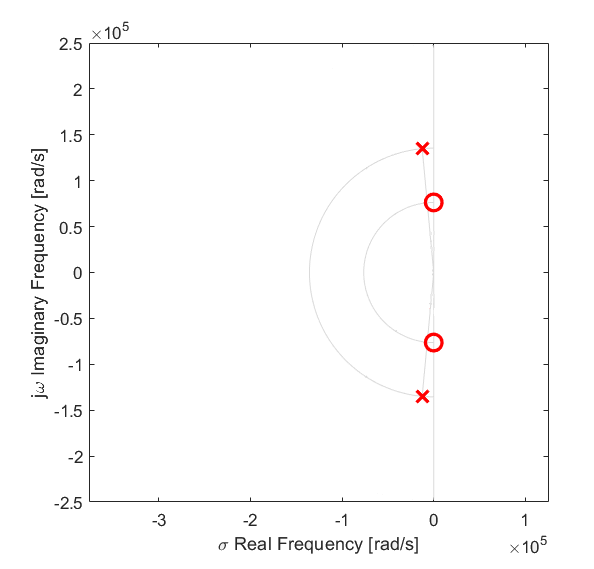
\includegraphics[width=0.5\textwidth]{../EJ3/Resources/polezero_stagei.png}
    \caption{Polos y ceros de la etapa I}
    \label{EJ3_PZEI}
\end{figure}

\begin{equation} 
\label{transf_stage2}
H_2(s) = \frac{s^2 + 1,175 \cdot 10^9}{s^2 + 2,668 \cdot 10^5 s + 2,473 \cdot 10^5}
\end{equation}

\begin{figure}[H] 
    \centering
    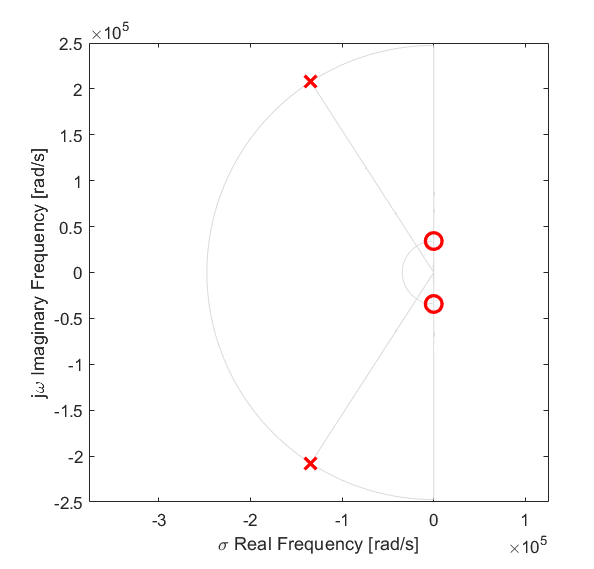
\includegraphics[width=0.5\textwidth]{../EJ3/Resources/polezero_stageii.png}
    \caption{Polos y ceros de la etapa II}
    \label{EJ3_PZEII}
\end{figure}

Se observa que ambas funciones transferencia responden a un comportamiento del tipo high pass notch, por lo que consultando la tabla~\ref{tabla_circuitos} se deriva que se utilizar\'a el circuito HPB.

Definido el tipo de circuito a utlizar, en lo subsiguiente se trata el dise\~no de cada etapa por separado.

\subsubsection{Dise\~no de etapa I}

La etapa I esta descripta por la funci\'on transferencia en \ref{transf_stage1}, de la que se derivan los valores de la tabla de abajo.

\begin{table}[H]
    \centering
    \begin{tabular}{c c}
        Par\'ametro & Valor\\
        \hline
         $\omega_0$ & $1,354 \cdot 10^5 \frac{rad}{s}$ \\
	     $\omega_z$ & $7,639 \cdot 10^4 \frac{rad}{s}$  \\
         $Q$ & $5,38$ \\
    \end{tabular}
    \caption{Especificaciones de etapa I}
    \label{tabla_stageI}
\end{table}



En primer lugar se debe elegir el valor de $Q_0$ acorde a la ecuaci\'on~\ref{q0}. Se determina $Q_0 = 2$. Luego, se calculan las constantes $k$, $K$, $m$ y $n$ con las siguientes f\'ormulas:

\begin{equation}
\label{eq_ck}
K = \frac{1}{2Q_0^2} \cdot \left( 1- \frac{Q_0}{Q}\right)
\end{equation}

\begin{equation}
\label{eq_k}
k = \frac{n_2 \left( \frac{\omega_z}{\omega_0}\right)^2}{\left(1-\frac{Q_0}{Q}\right)}
\end{equation}

\begin{equation}
\label{eq_n}
n = k \cdot \left( 1-\frac{Q_0}{KQ}\right)
\end{equation}

\begin{equation}
\label{eq_m}
m = k\cdot \left( \frac{K-1}{K}\right) \cdot \left[ 1+2Q_0^2\left(\frac{\omega_0}{\omega_z}\right)^2\right]
\end{equation}

Obteniendo los siguientes valores

\begin{table}[H]
    \centering
    \begin{tabular}{c c}
        Constante & Valor\\
        \hline
         $K$ & $1,0785$ \\
	     $k$ & $0,50506$  \\
         $n$ & $0,3309$ \\
         $m$ & $0,9639$ \\
    \end{tabular}
    \caption{Constantes de etapa I}
    \label{tabla_stageI_ctes}
\end{table}

Con estas constantes se realizan las estimaciones de abajo

\begin{equation}
\frac{C_{22}}{C_{21}} \approx \frac{m}{1-m} \approx 26,748
\end{equation}

\begin{equation}
C_3 \approx C_{21}+C_{22}\approx 27,748 \cdot C_{21}
\end{equation}

Luego, se fijan $C_{21} = 1nF$ y $C_{22} = C_3 = 27nF$.
Por otro lado, empleando las ecuaciones~\ref{omega_predistortion} y \ref{q_predistortion} se obtienen $\omega_p = 1,3694 \cdot 10^5 \frac{rad}{s}$ y $Q_p = 5,227$. Realizado esto se emplean las formulas que se reproducen a continuaci\'on para calcular $G_1$ y $G_{41} + G_{42}$.

\begin{equation}
\label{g1}
G_1 = 2Q_0\omega_p\sqrt{C_3\left(C_{21}+C_{22}\right)}
\end{equation}

\begin{equation}
\label{g41+g42}
G_{41} + G_{42} = \frac{G_1}{4Q_0^2}
\end{equation}

Resultando $G_1 = 1,5 \cdot 10^{-2}s$ y $G_{41}+G_{42}=9,413\cdot 10^-4s$.

Por otro lado se determina arbitrariamente un valor para $G_b$, y con la relaci\'on de abajo se hace lo propio con $G_{a1} + G_{a2}$.

\begin{equation}
\frac{G_{a1} + G_{a2}}{G_b} = \left( \frac{G_{41}+G_{42}}{G_1}\right) \left( \frac{C_{21}+C_{22}+C_3}{C_3}\right) \approx 0,07861
\end{equation}

Se toma $R_b = 47k\Omega$. Luego, con se iguala la ecuaci\'on~\ref{hpbn1} ($n_1$) a cero y se obtiene una relaci\'on entre $G_{a2}$ y $G_{42}$. La otra relaci\'on se obtiene dividiendo las ecuaciones \ref{hpbn0} y \ref{hpbn1}, y reemplazando el cociente $\frac{n_0}{n_1}$ por $\omega_z^2$.



Finalmente, se obtienen los siguientes valores para los componentes del circuito. Para minimizar el error se emplean varios componentes en serie y paralelo, de tal forma de lograr minimizar el error.


\begin{table}[H]
    \centering
    \begin{tabular}{c c c c}
        Componente & Valor te\'orico & Valor real & Error\\
        \hline
         $G_1$ & $66,4\Omega$ & $66\Omega (56\Omega + 10\Omega)$ & $0,6\%$ \\
	     $G_b$ & $47k\Omega$ & $47k\Omega$ & $0\%$ \\
         $G_{42}$ & $3,268k\Omega$ & $3,260k\Omega (2,7k\Omega + 560\Omega)$ & $0,2\%$ \\
         $G_{41}$ & $1,573k\Omega$ & $1,568k\Omega (1,5k\Omega+68\Omega)$ & $0,4\%$ \\
         $G_{a2}$ & $1,186M\Omega$ & $1,2M\Omega$ & $1,1\%$ \\
	     $G_{a1}$ & $1,204M\Omega$ & $1,2M\Omega$ & $0,4\%$ \\
         $C_{21}$ & $1nF$ & $1nF$ & $0\%$ \\
         $C_{22}$ & $26,7nF$ & $27nF$ & $0,9\%$ \\
         $C_3$ & $27,7nF$ & $27nF$ & $2,7\%$ \\
    \end{tabular}
    \caption{Componentes de etapa I}
    \label{tabla_stageI_comp}
\end{table}

\begin{figure}[H]
    \centering
    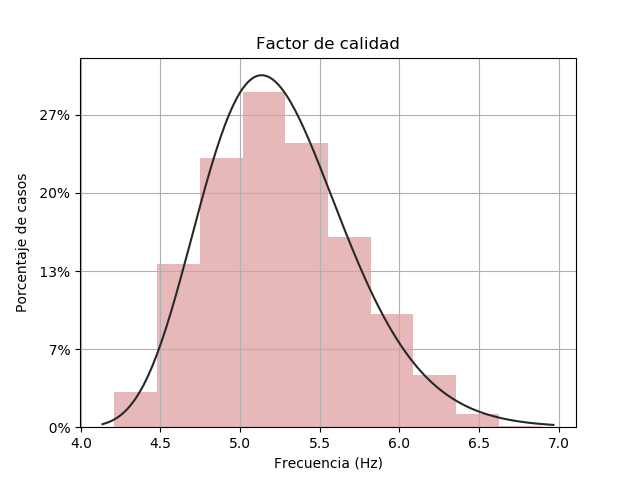
\includegraphics[width=0.6\textwidth]{../EJ3/Resources/histograma_stagei.png}
    \caption{Histograma de etapa I}
     \label{EJ3_STAGEI_HIST}
\end{figure}


Luego, se compara lo simulado con lo medido en la primera etapa.

\begin{figure}[H]
    \centering
    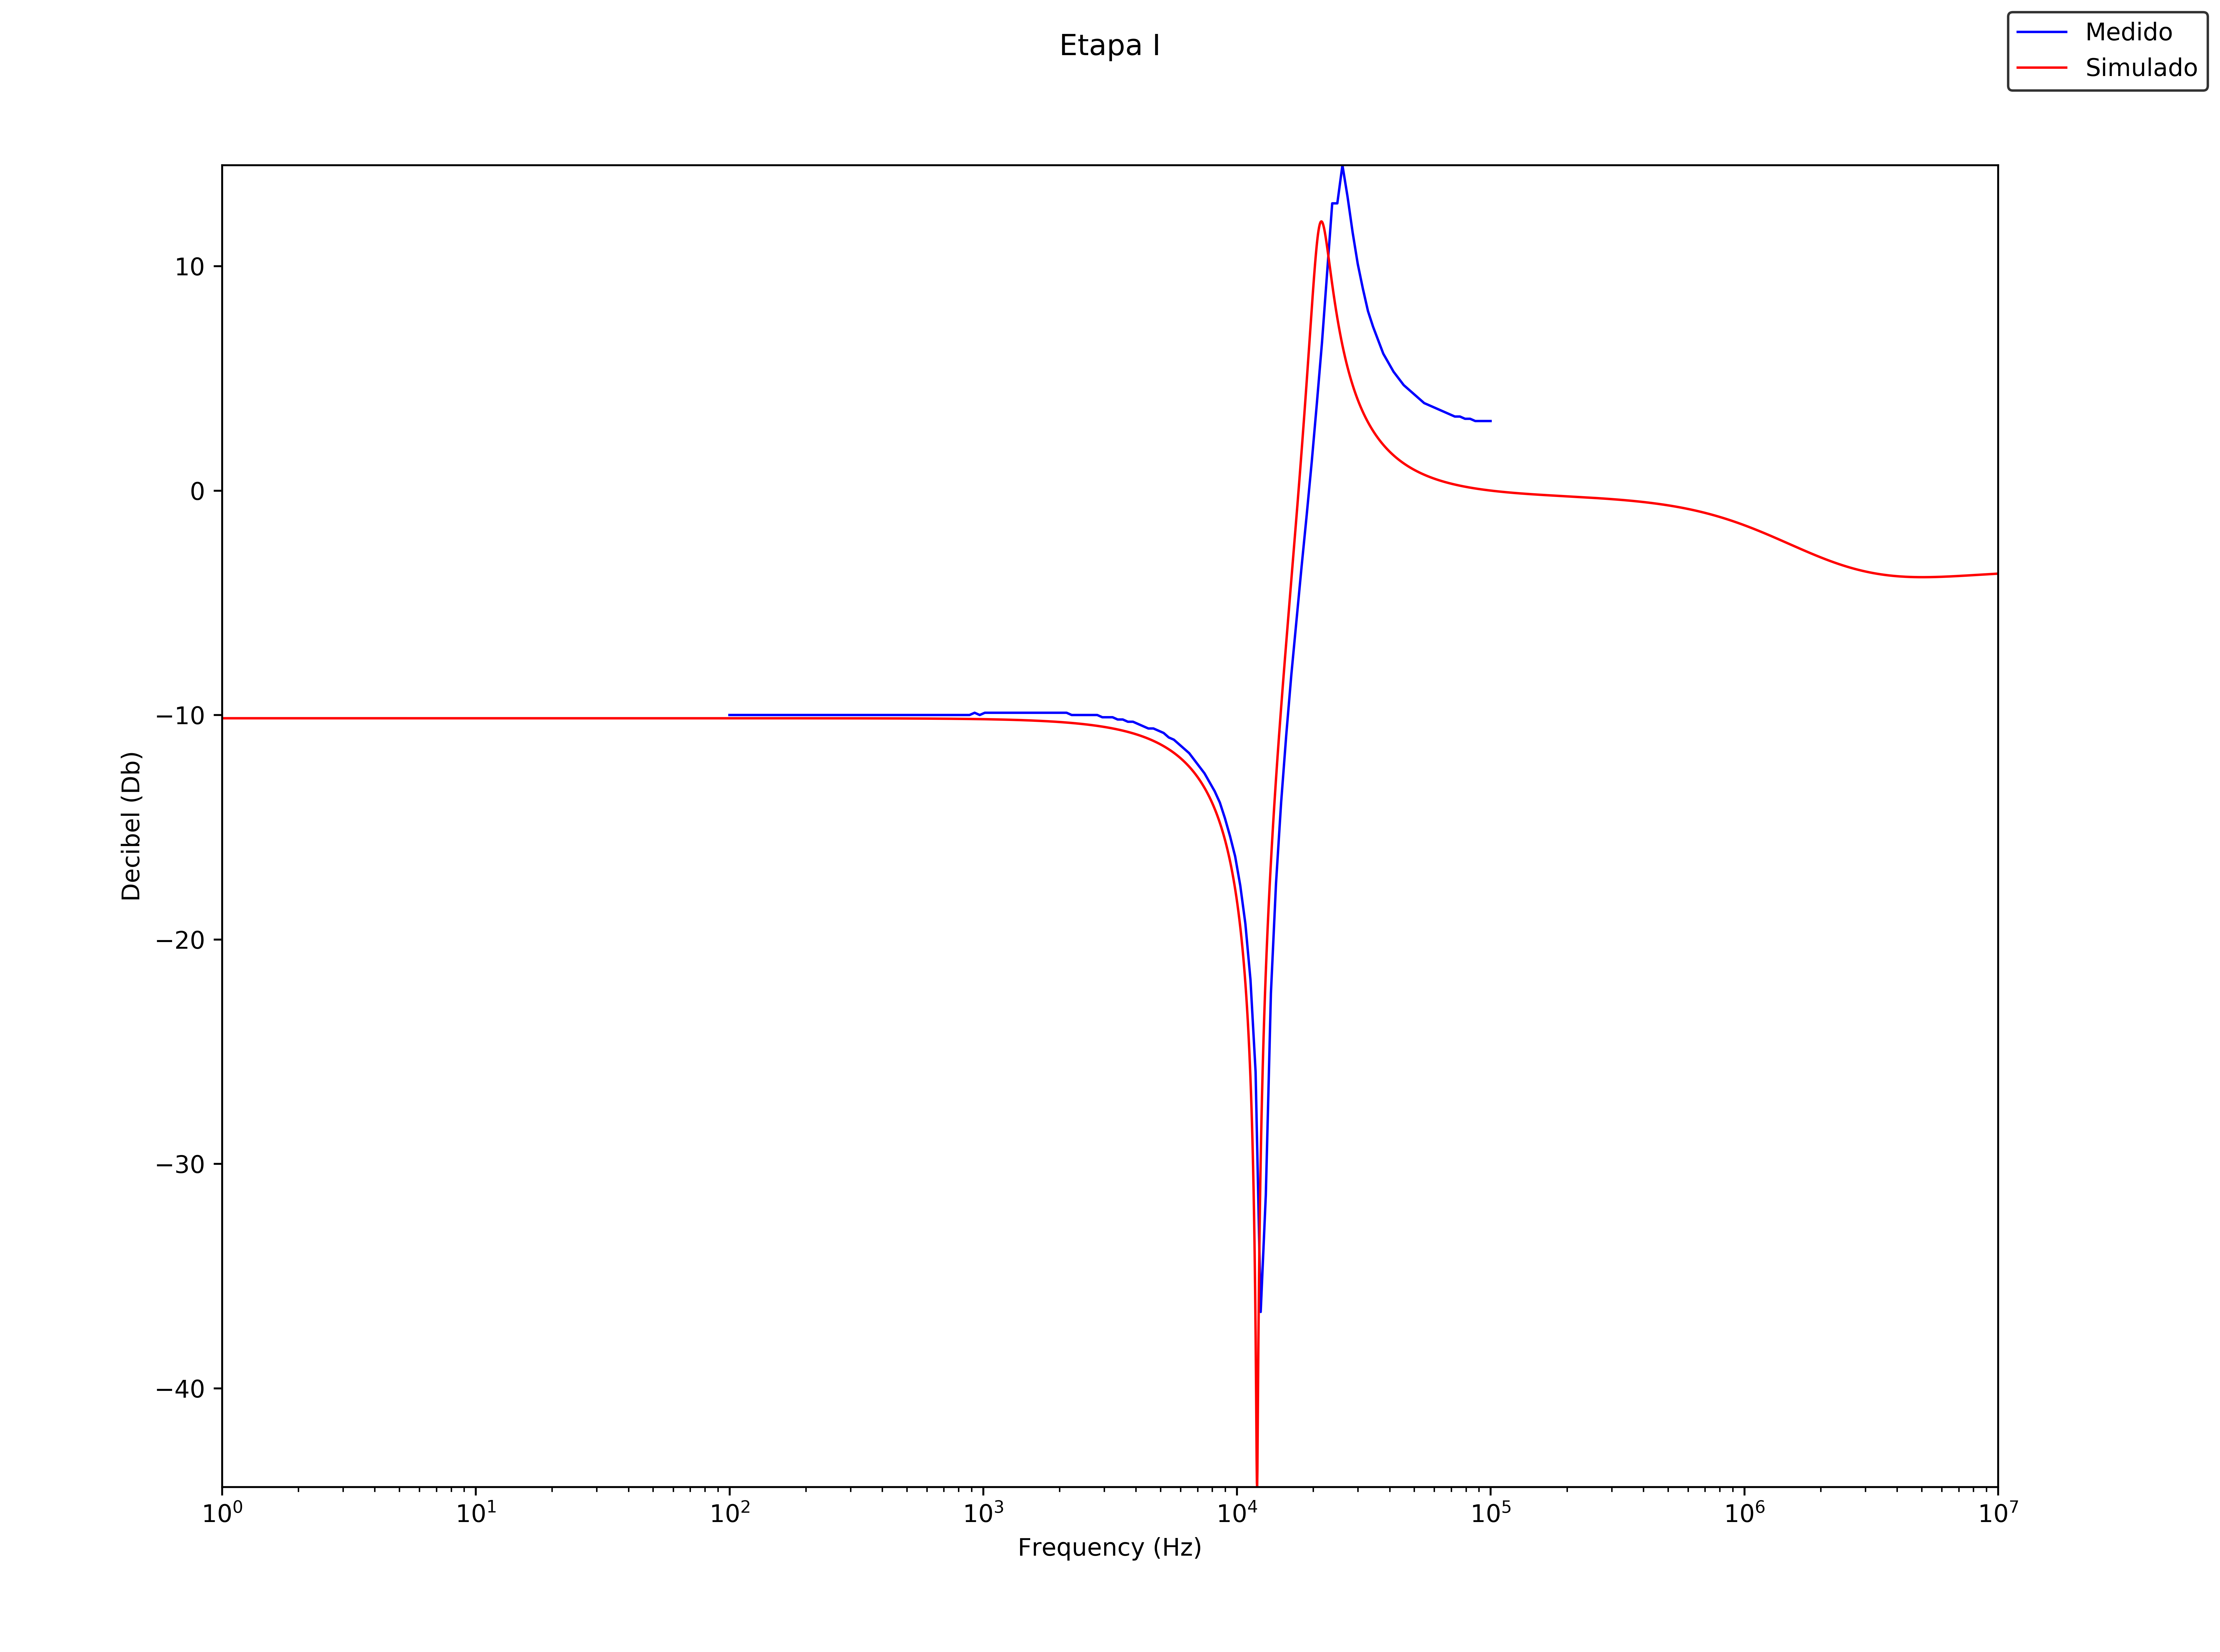
\includegraphics[width=0.9\textwidth]{../EJ3/Resources/stageI_ampbode.png}
    \caption{Etapa I - Diagrama BODE de m\'odulo}
     \label{EJ3_STAGEI_BODEAMP}
\end{figure}

\begin{figure}[H]
    \centering
    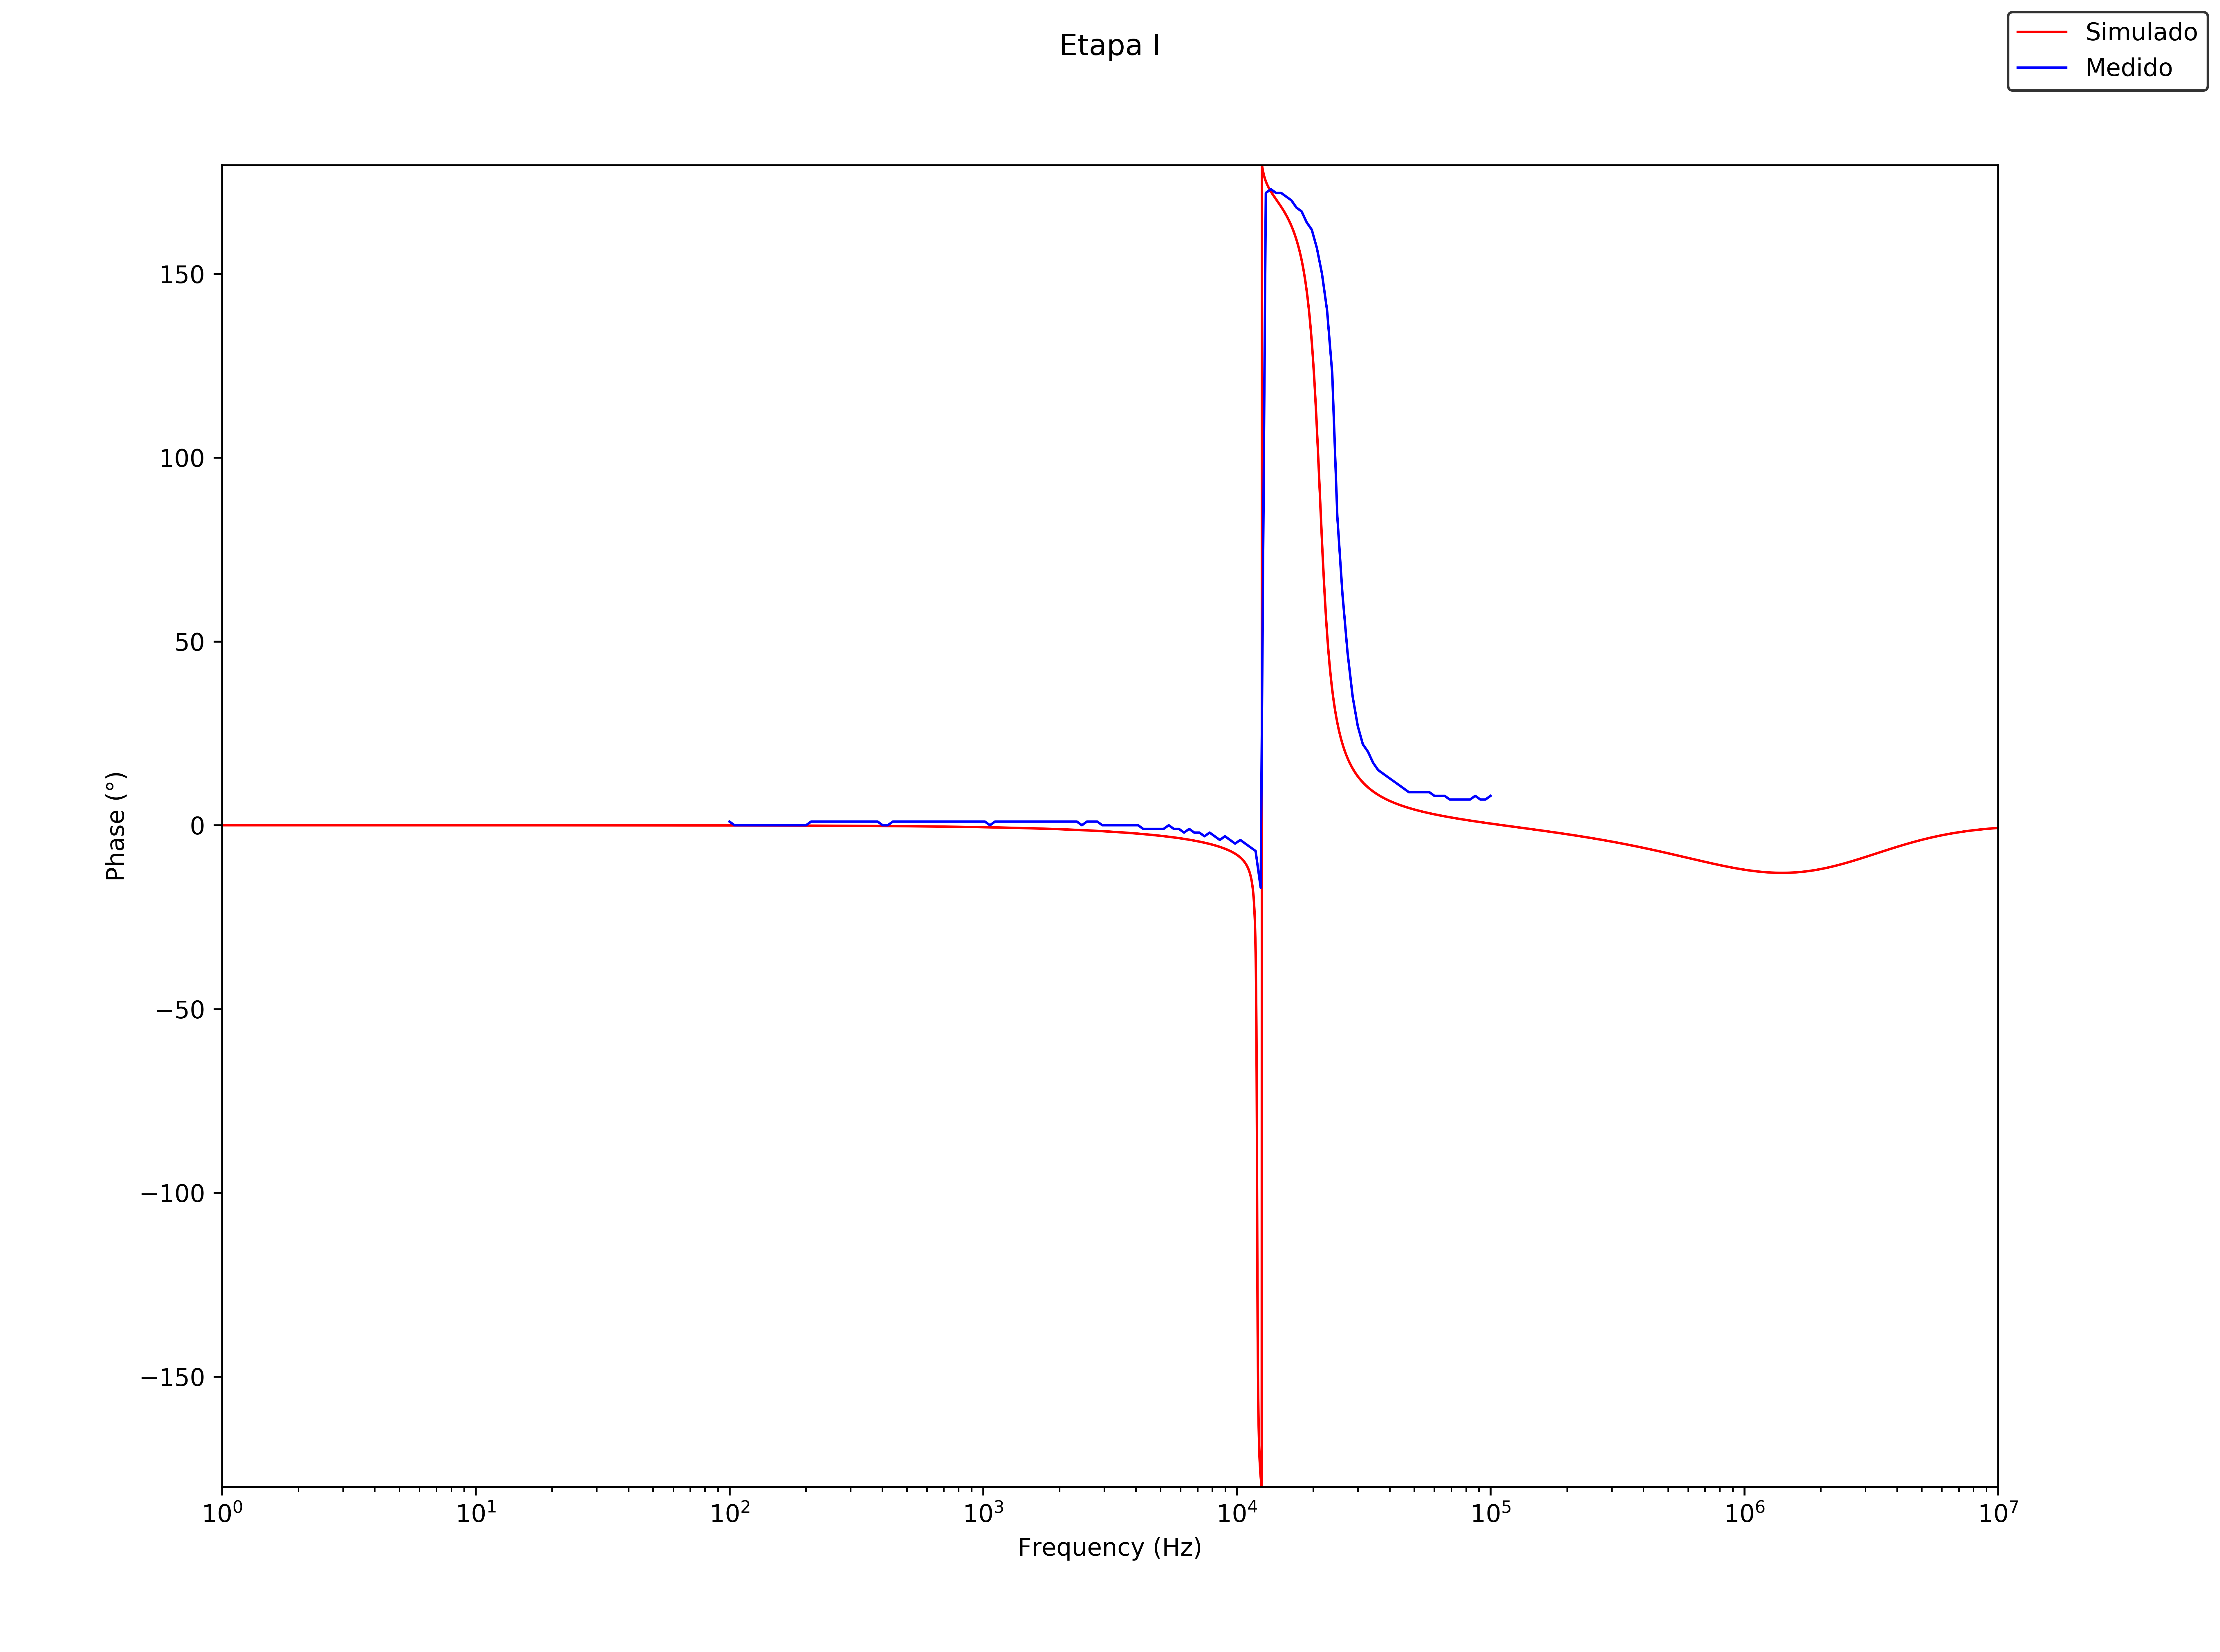
\includegraphics[width=0.9\textwidth]{../EJ3/Resources/stageI_phabode.png}
    \caption{Etapa I - Diagrama BODE de fase}
     \label{EJ3_STAGEI_BODEPHA}
\end{figure}

Las sensibilidades de la etapa estar\'an dadas por la siguiente tabla.

\begin{table}[H]
    \centering
    \begin{tabular}{c | c c}
         & $\omega_0$ & Q\\
        \hline
        $R_1$  & $-\frac{1}{2}$ & $-2,19$ \\
        $C_2$  & $-\frac{1}{2}$ & $-0,845$ \\
        $C_3$  & $-\frac{1}{2}$ & $0,845$\\
        $R_4$  & $-\frac{1}{2}$ & $2,19$ \\
        $R_a$  & $0$ & $-1,69$\\
        $R_b$  & $0$ & $1,69$\\
    \end{tabular}
    \caption{Sensibilidades pasivas de etapa I}
    \label{tabla_sensibilidades_pasivas_stageI}
\end{table}

\subsubsection{Dise\~no de etapa II}

El dise\~no de la segunda etapa sigue la misma l\'ogica que el de la precedente, por lo que no se cree necesario su desarrollo. Las especificaciones de dicha etapa est\'an identificadas en la ecuaci\'on~\ref{transf_stage2}, y adem\'as se reproducen en la siguiente tabla.

\begin{table}[H]
    \centering
    \begin{tabular}{c c}
        Par\'ametro & Valor\\
        \hline
         $\omega_0$ & $2,473 \cdot 10^5 \frac{rad}{s}$ \\
	     $\omega_z$ & $3,427 \cdot 10^4 \frac{rad}{s}$  \\
         $Q$ & $0,92$ \\
    \end{tabular}
    \caption{Especificaciones de etapa II}
    \label{tabla_stageI}
\end{table}

Se fija el par\'ametro $Q_0 = 0,4$. A partir de esto se calculan los coeficientes. 

\begin{table}[H]
    \centering
    \begin{tabular}{c c}
        Constante & Valor\\
        \hline
         $K$ & $2,7663$ \\
	     $k$ & $0,0339$  \\
         $n$ & $0,0286$ \\
         $m$ & $0,3831$ \\
    \end{tabular}
    \caption{Constantes de etapa II}
    \label{tabla_stageII_ctes}
\end{table}

Luego del mismo razonamiento que en la primera etapa, llega a los valores de componentes ideales para la construcci\'on de la celda.


\begin{table}[H]
    \centering
    \begin{tabular}{c c c c}
        Componente & Valor te\'orico & Valor real & Error\\
        \hline
         $G_1$ & $194\Omega$ & $195\Omega (180\Omega + 15\Omega)$ & $0,5\%$ \\
	     $G_b$ & $47k\Omega$ & $47k\Omega$ & $0\%$ \\
         $G_{42}$ & $2,717k\Omega$ & $2,718k\Omega (2,7k\Omega + 18\Omega)$ & $0,02\%$ \\
         $G_{41}$ & $130,1\Omega$ & $130\Omega (120\Omega+10\Omega)$ & $0,10\%$ \\
         $G_{a2}$ & $490,89k\Omega$ & $492k\omega (470k\Omega+22k\Omega)$ & $0,22\%$ \\
	     $G_{a1}$ & $28,167k\Omega$ & $28,2k\Omega (27k\Omega + 1,2k\Omega)$ & $0,12\%$ \\
         $C_{21}$ & $10nF$ & $10nF$ & $0\%$ \\
         $C_{22}$ & $16,1nF$ & $16nF (15nF + 1nF)$ & $0,6\%$ \\
         $C_3$ & $26,1nF$ & $25,9nF (22nF + 3,9nF)$ & $0,8\%$ \\
    \end{tabular}
    \caption{Componentes de etapa II}
    \label{tabla_stageII_comp}
\end{table}

\begin{figure}[H]
    \centering
    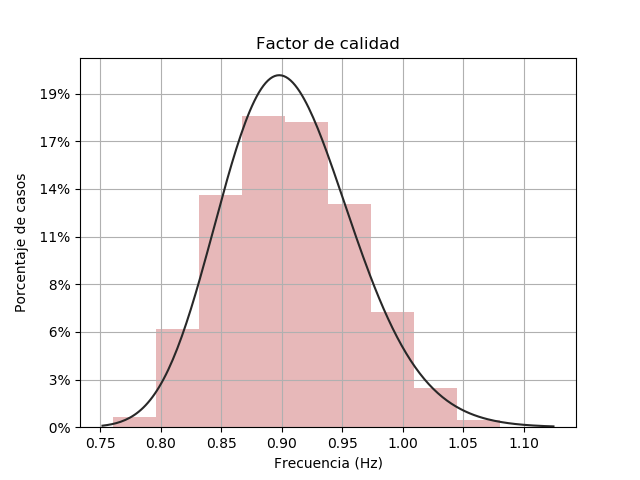
\includegraphics[width=0.6\textwidth]{../EJ3/Resources/histograma_stageii.png}
    \caption{Histograma de etapa II}
     \label{EJ3_STAGEII_HIST}
\end{figure}

A partir de esto se realiza la simulaci\'on del circuito, y se lo compara con lo medido en la pr\'actica.

\begin{figure}[H]
    \centering
    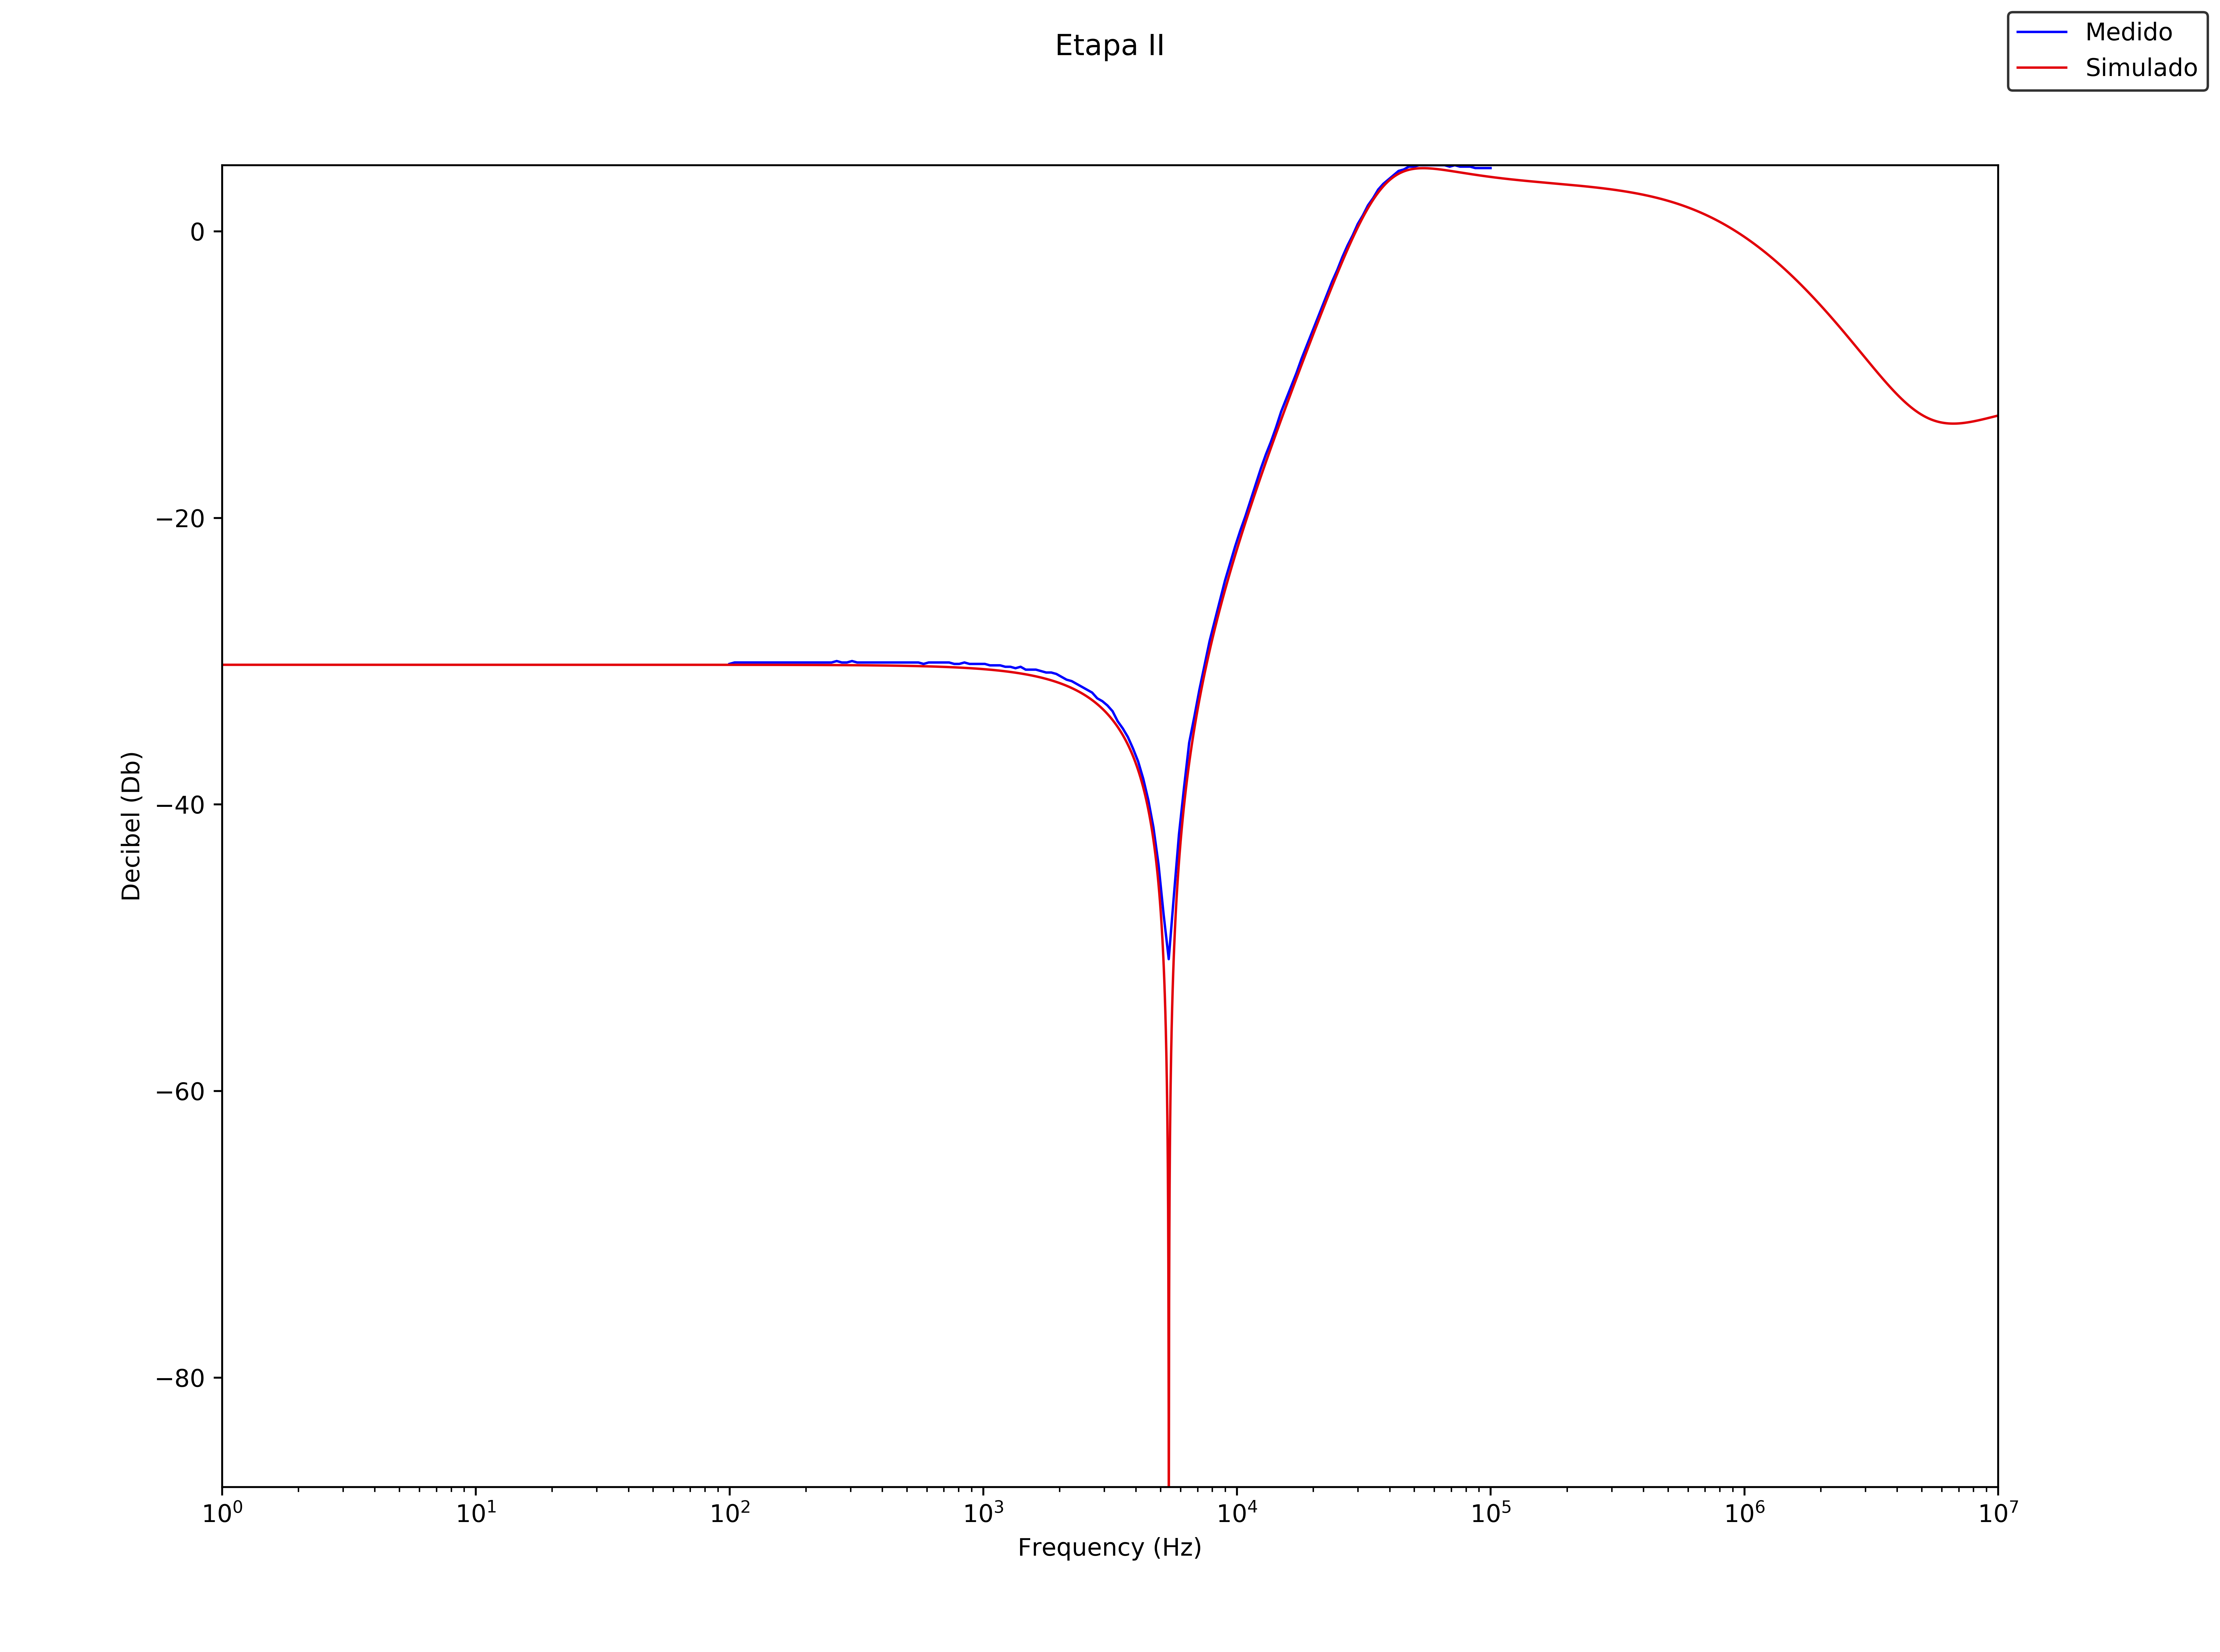
\includegraphics[width=0.9\textwidth]{../EJ3/Resources/stageII_ampbode.png}
    \caption{Etapa II - Diagrama BODE de m\'odulo}
     \label{EJ3_STAGEII_BODEAMP}
\end{figure}

\begin{figure}[H]
    \centering
    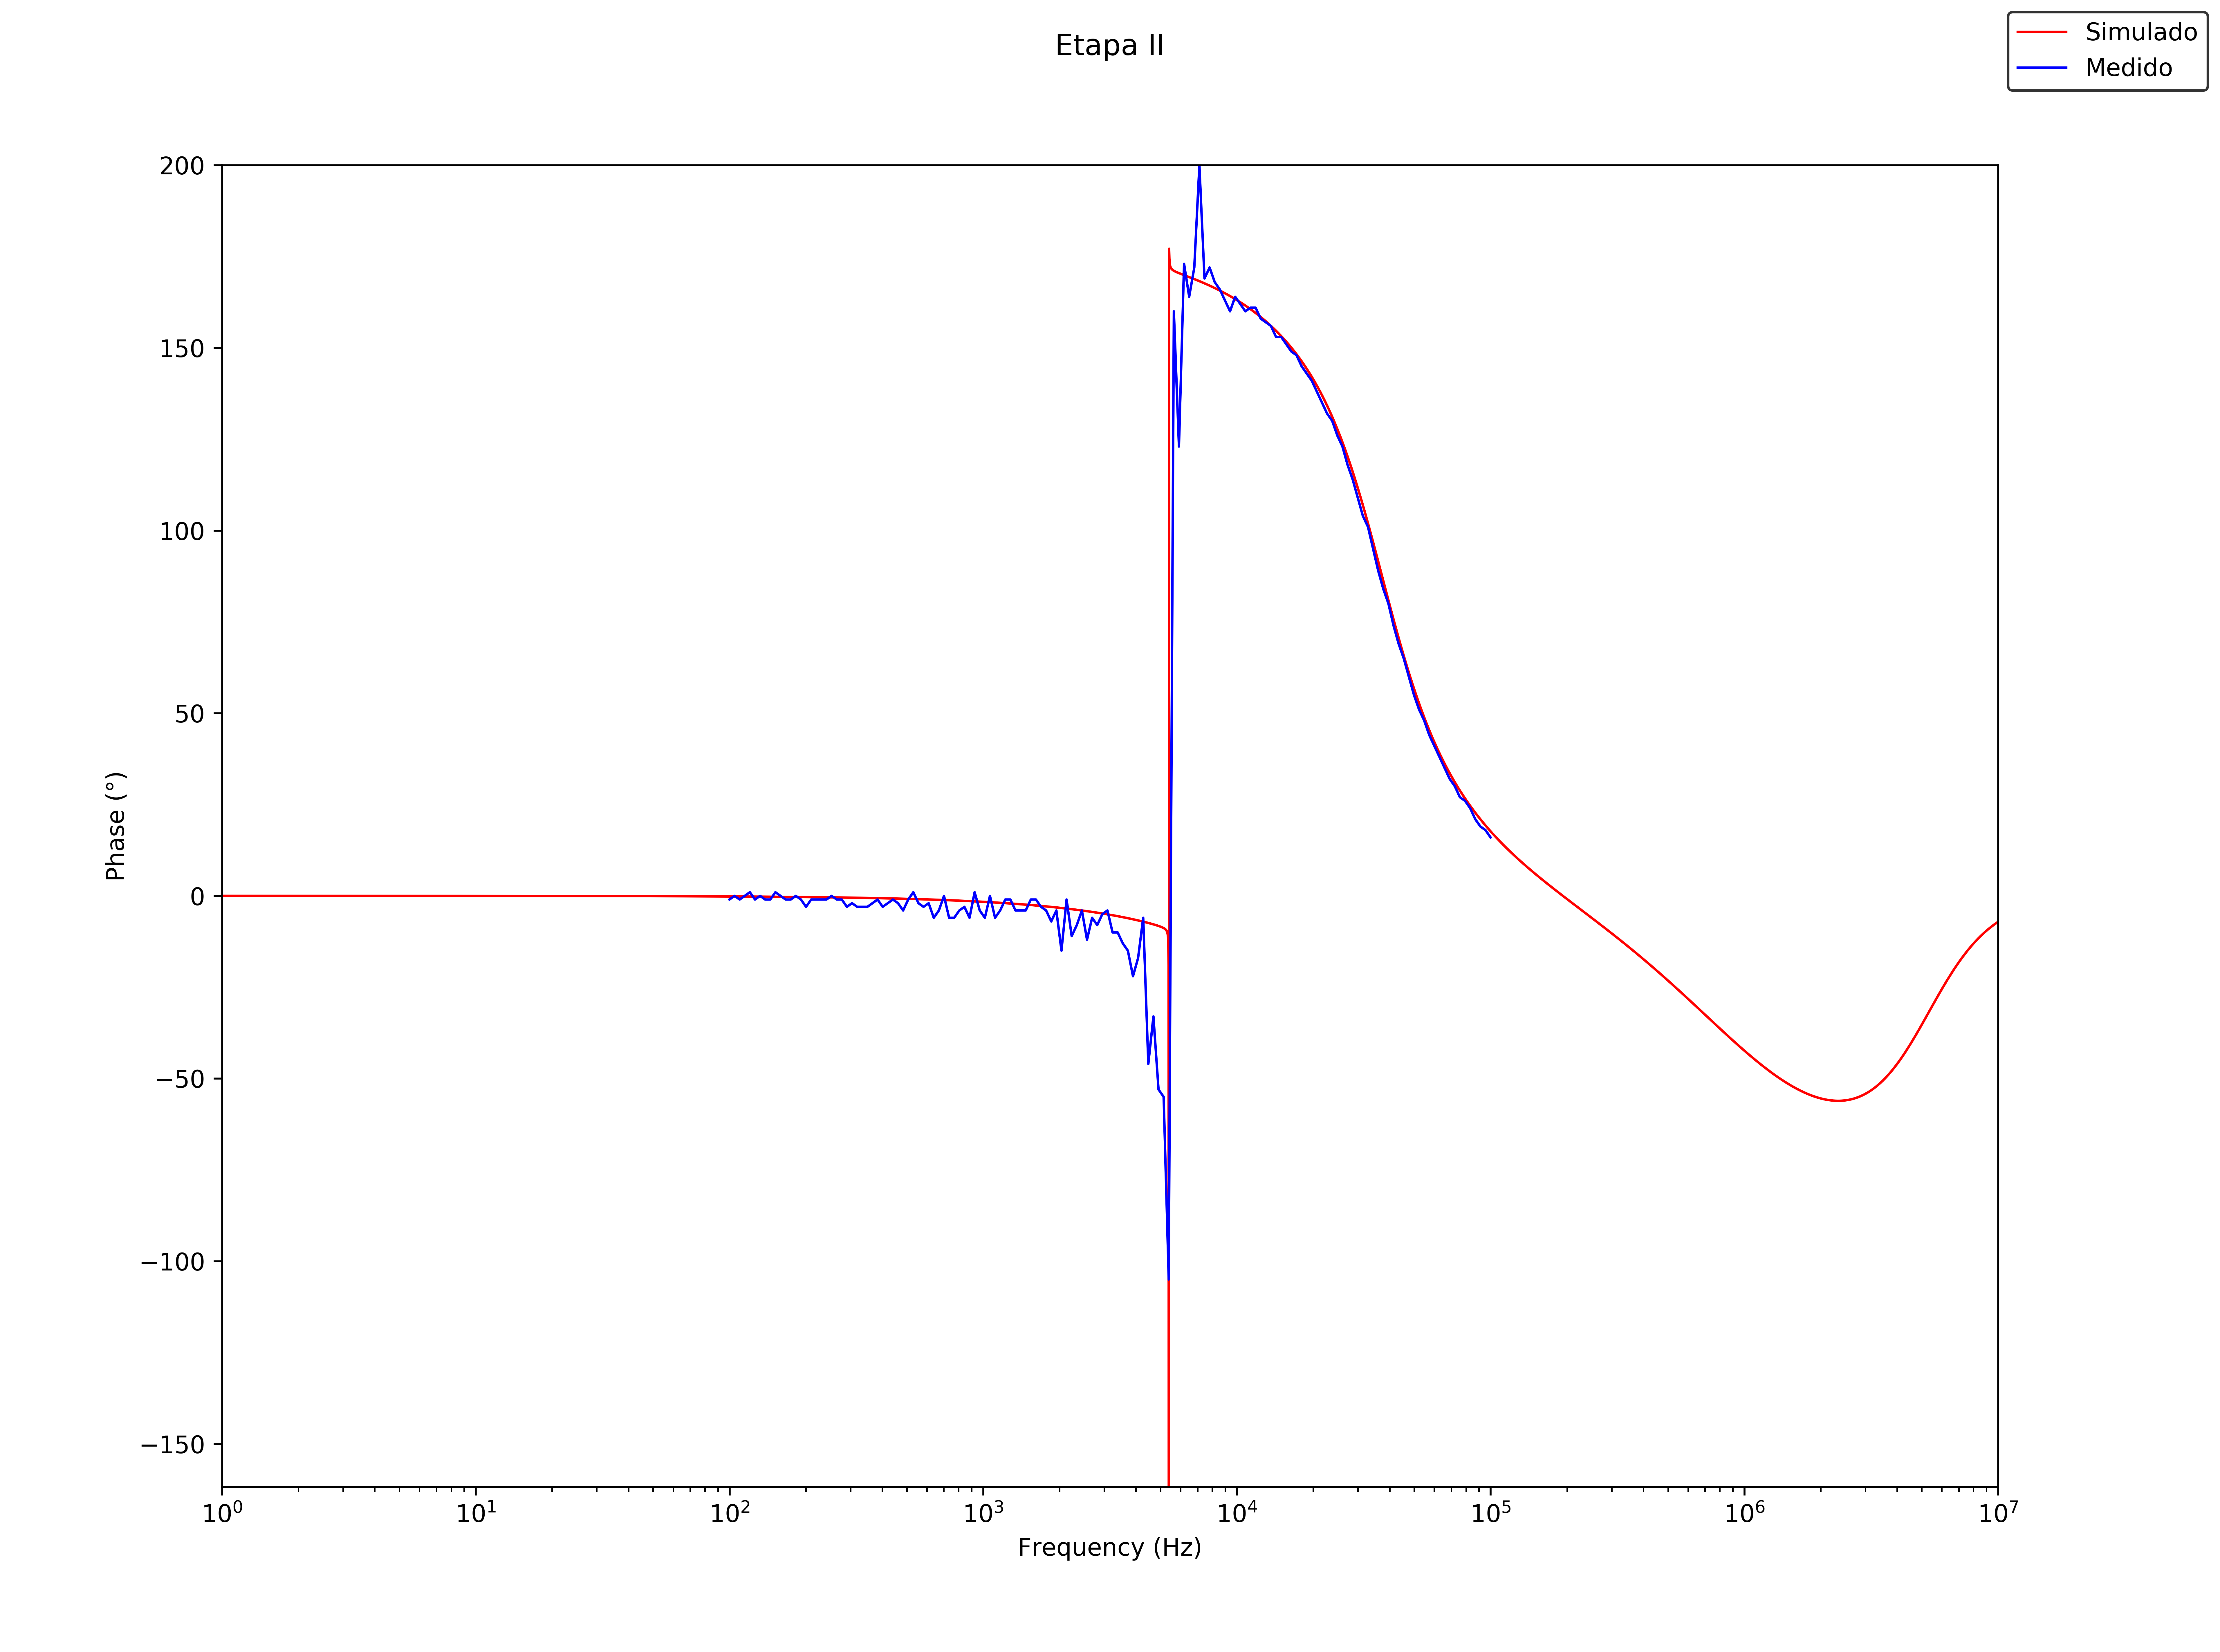
\includegraphics[width=0.9\textwidth]{../EJ3/Resources/stageII_phabode.png}
    \caption{Etapa II - Diagrama BODE de fase}
     \label{EJ3_STAGEII_BODEPHA}
\end{figure}

Las sensibilidades de la etapa II ser\'an

\begin{table}[H]
    \centering
    \begin{tabular}{c | c c}
         & $\omega_0$ & Q\\
        \hline
        $R_1$  & $-\frac{1}{2}$ & $-2,19$ \\
        $C_2$  & $-\frac{1}{2}$ & $-0,845$ \\
        $C_3$  & $-\frac{1}{2}$ & $0,845$\\
        $R_4$  & $-\frac{1}{2}$ & $2,19$ \\
        $R_a$  & $0$ & $-1,69$\\
        $R_b$  & $0$ & $1,69$\\
    \end{tabular}
    \caption{Sensibilidades pasivas de etapa II}
    \label{tabla_sensibilidades_pasivas_stageII}
\end{table}

Los valores de sensibilidad de ambas etapas son los mismos debido a que se busc\'o que los $Q_0$ sean proporcionales a los $Q$ de las etapas.
En principio queda definido el circuito que constituye el filtro. El \'ultimo requerimiento a satisfacer es verificar que la impedancia de entrada del circuito no sea inferior a $50k\Omega$.

\subsubsection{Impedancia de entrada}

Ya realizado el dise\~no se obtiene el siguiente circuito.

\begin{figure}[H]
    \centering
    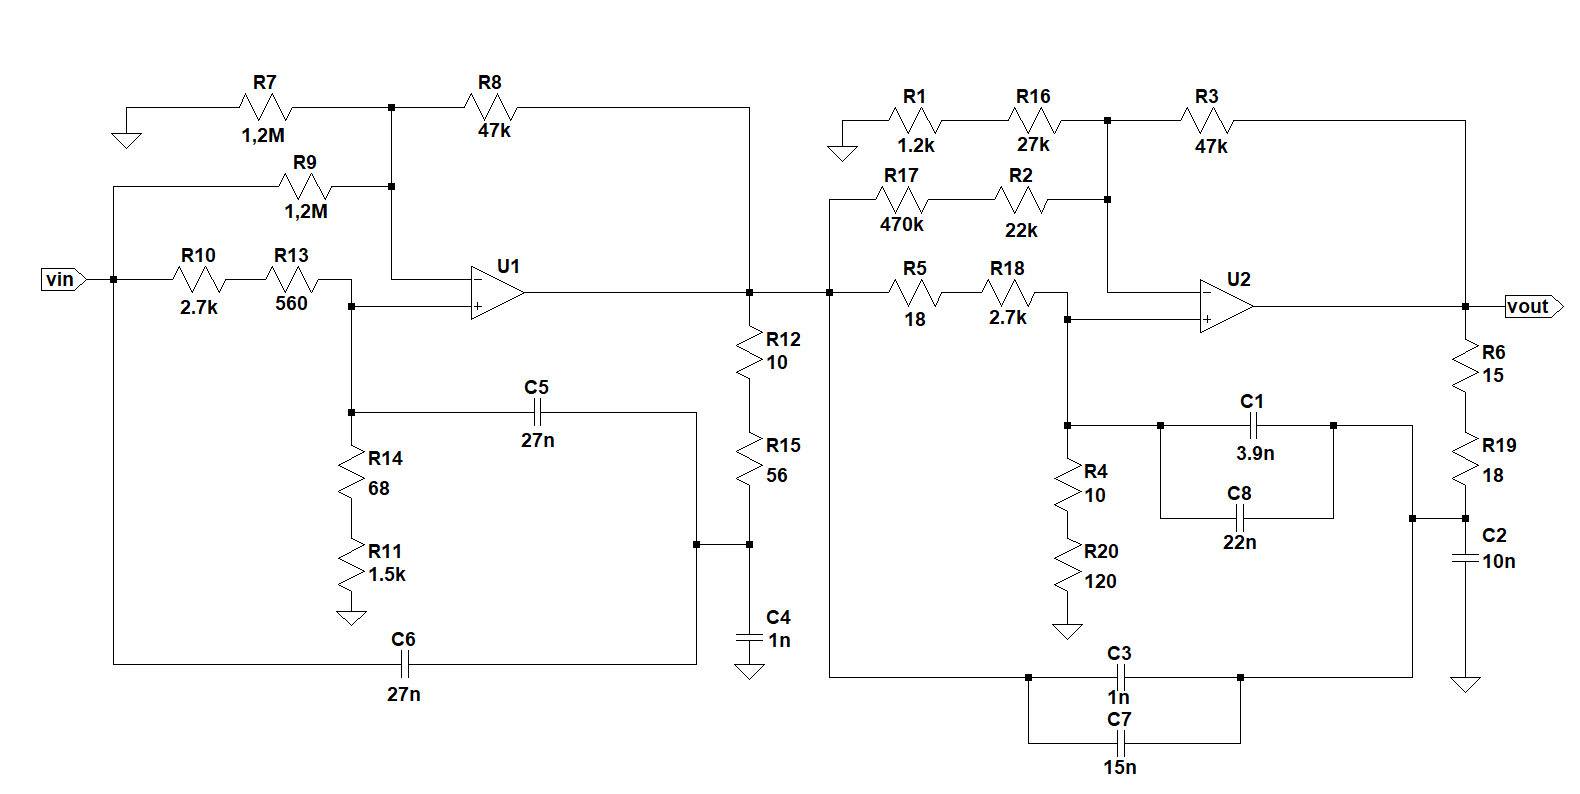
\includegraphics[width=0.9\textwidth]{../EJ3/Resources/filter_unbuffered.png}
    \caption{Circuito del filtro}
     \label{EJ3_FILTER_CIRCUIT_UNBUFFERED}
\end{figure}

Luego, se procede a realizar un diagrama montecarlo de las dos etapas acopladas, observando la impedancia de entrada del circuito en funci\'on de la frecuencia. Cabe destacar que para este ensayo se suponen en 1\% las tolerancias en los resistores, y un 15\% en el caso de capacitores.

\begin{figure}[H]
    \centering
    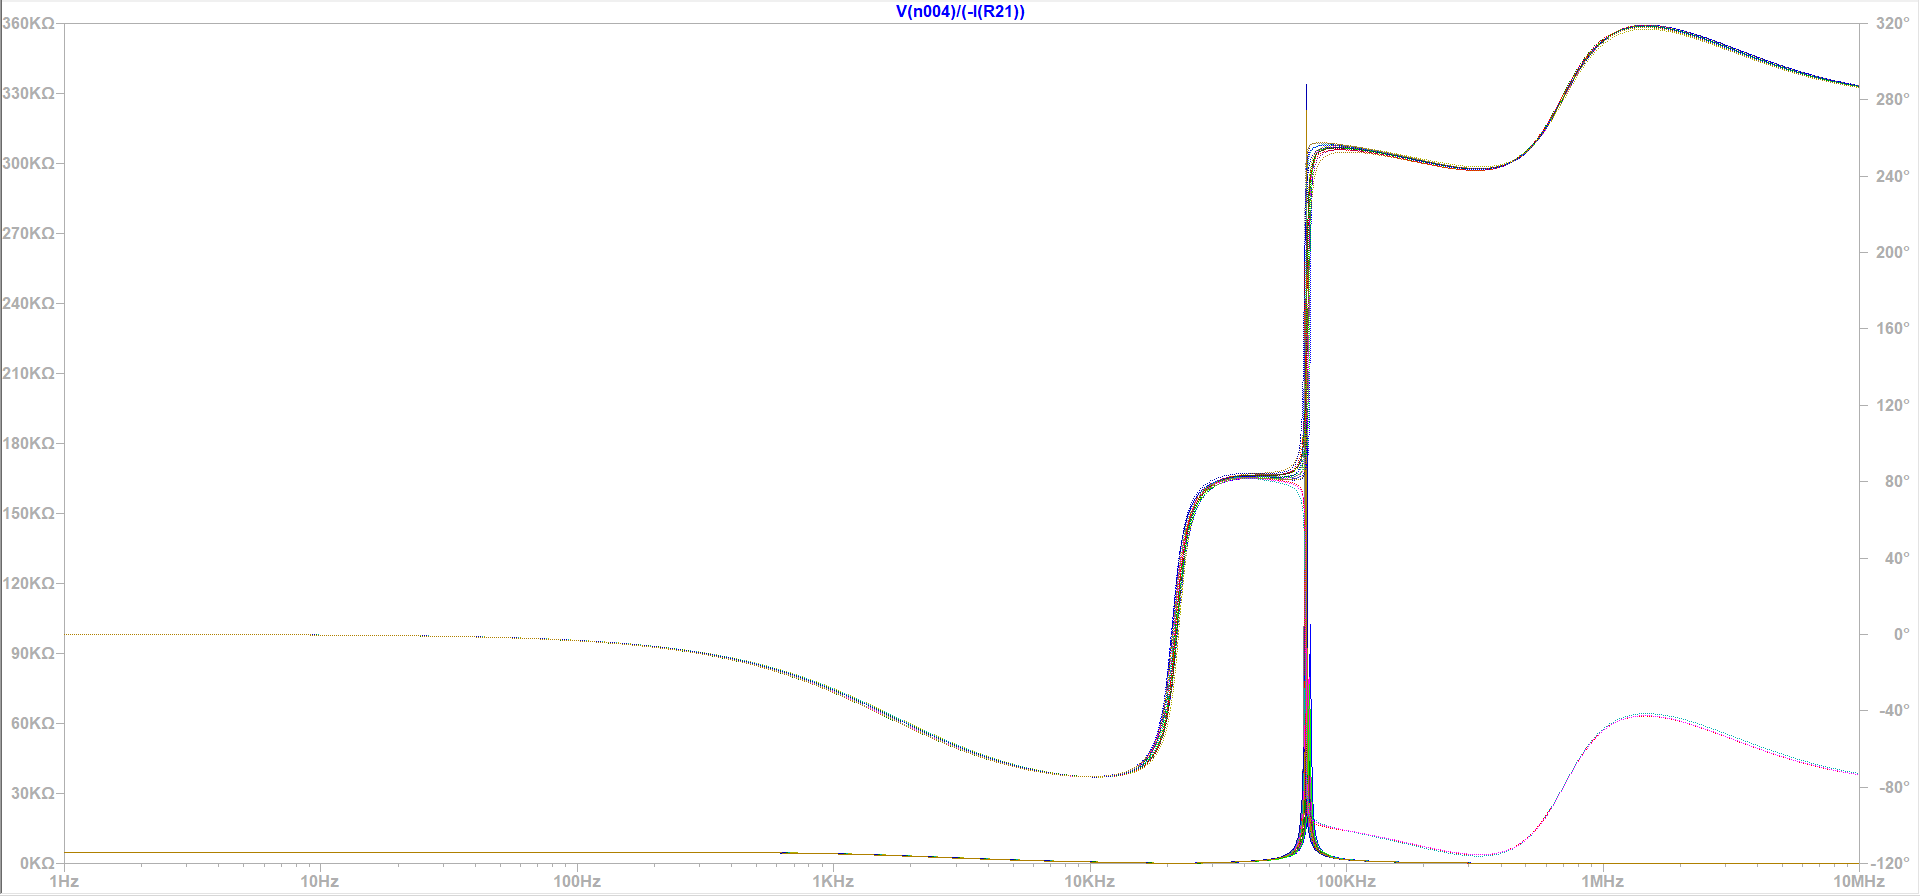
\includegraphics[width=0.9\textwidth]{../EJ3/Resources/zin_unbuffered.png}
    \caption{Impedancia de entrada del filtro}
     \label{EJ3_FILTER_ZIN_NOBUFF}
\end{figure}

Como se puede observar en el gr\'afico anterior, en frecuencias por debajo de $100kHz$ la impedancia de entrada del circuito no satisface la condici\'on requerida. Por lo tanto, se decide colocar un buffer a la entrada del filtro, as\'i como hacer lo mismo entre etapas. De esta forma se aumenta notablemente la impedancia de entrada, haciendo al filtro menos suceptible a ser cargado por una etapa posterior. El resultado se muestra en el gr\'afico subsiguiente.

\begin{figure}[H]
    \centering
    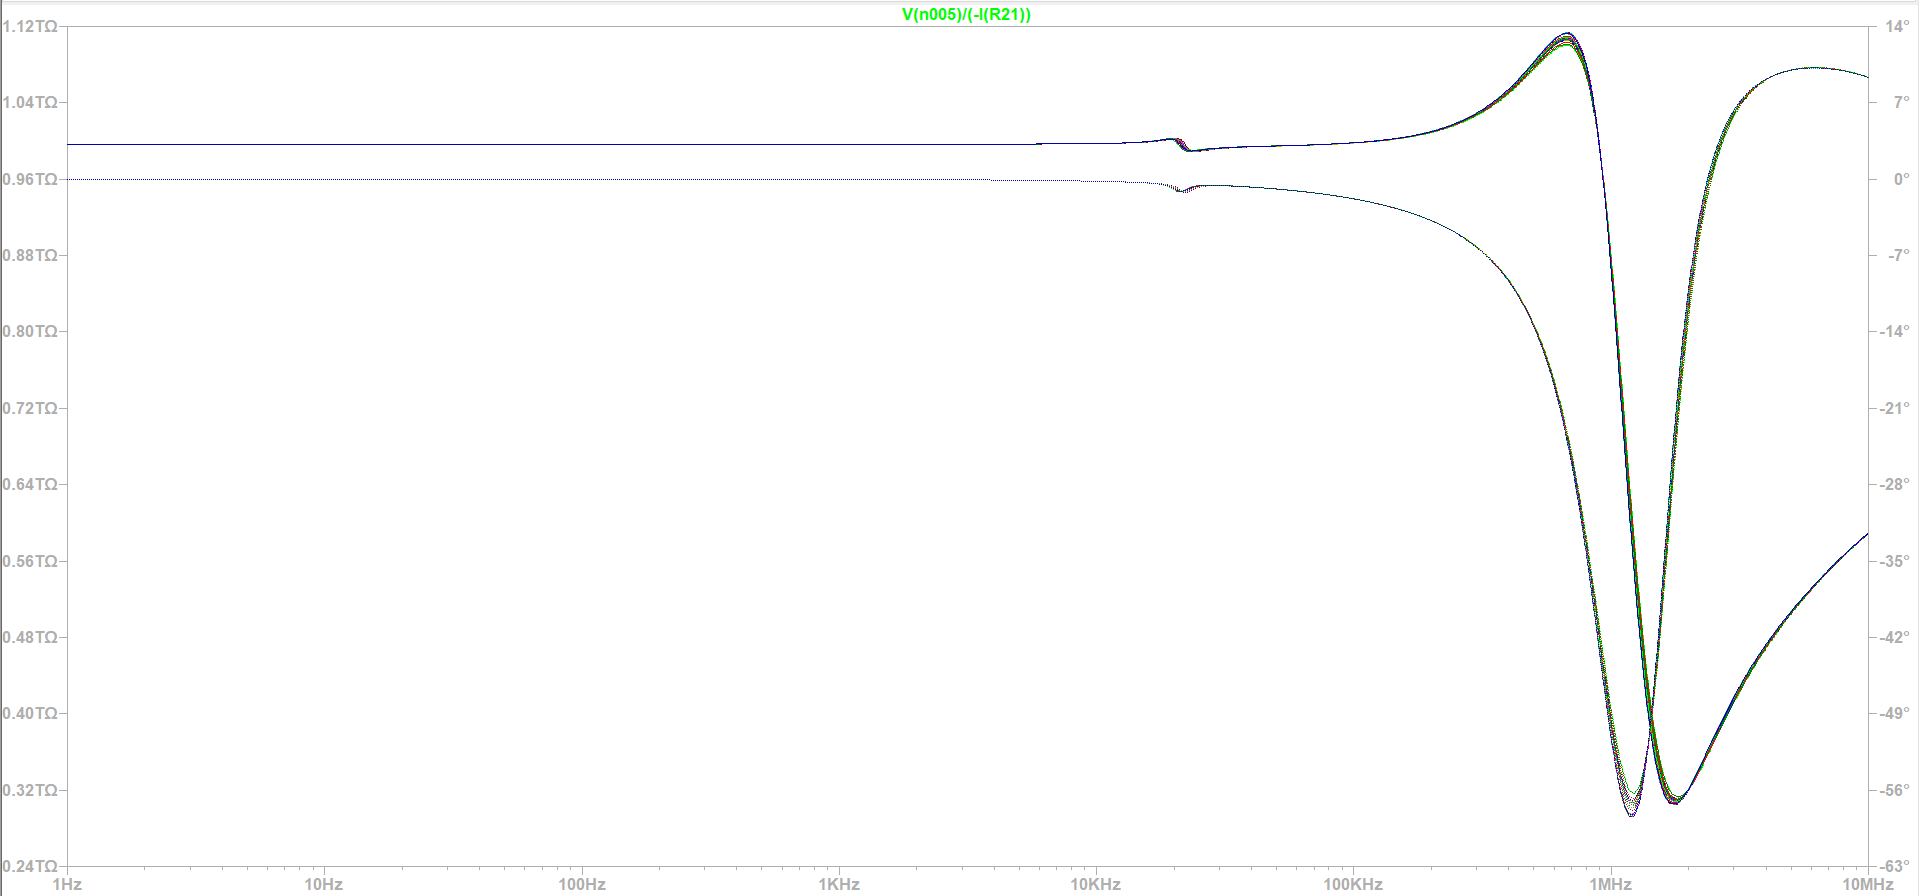
\includegraphics[width=0.9\textwidth]{../EJ3/Resources/zin_buffered.png}
    \caption{Impedancia de entrada del filtro empleando buffers}
     \label{EJ3_FILTER_ZIN_BUFFERED}
\end{figure}

Se advierte que con el agregado de estos dispositivos el cambio en la impedancia de entrada del filtro es notable. Finalmente, se obtiene el siguiente circuito para el filtro.


\begin{figure}[H]
    \centering
    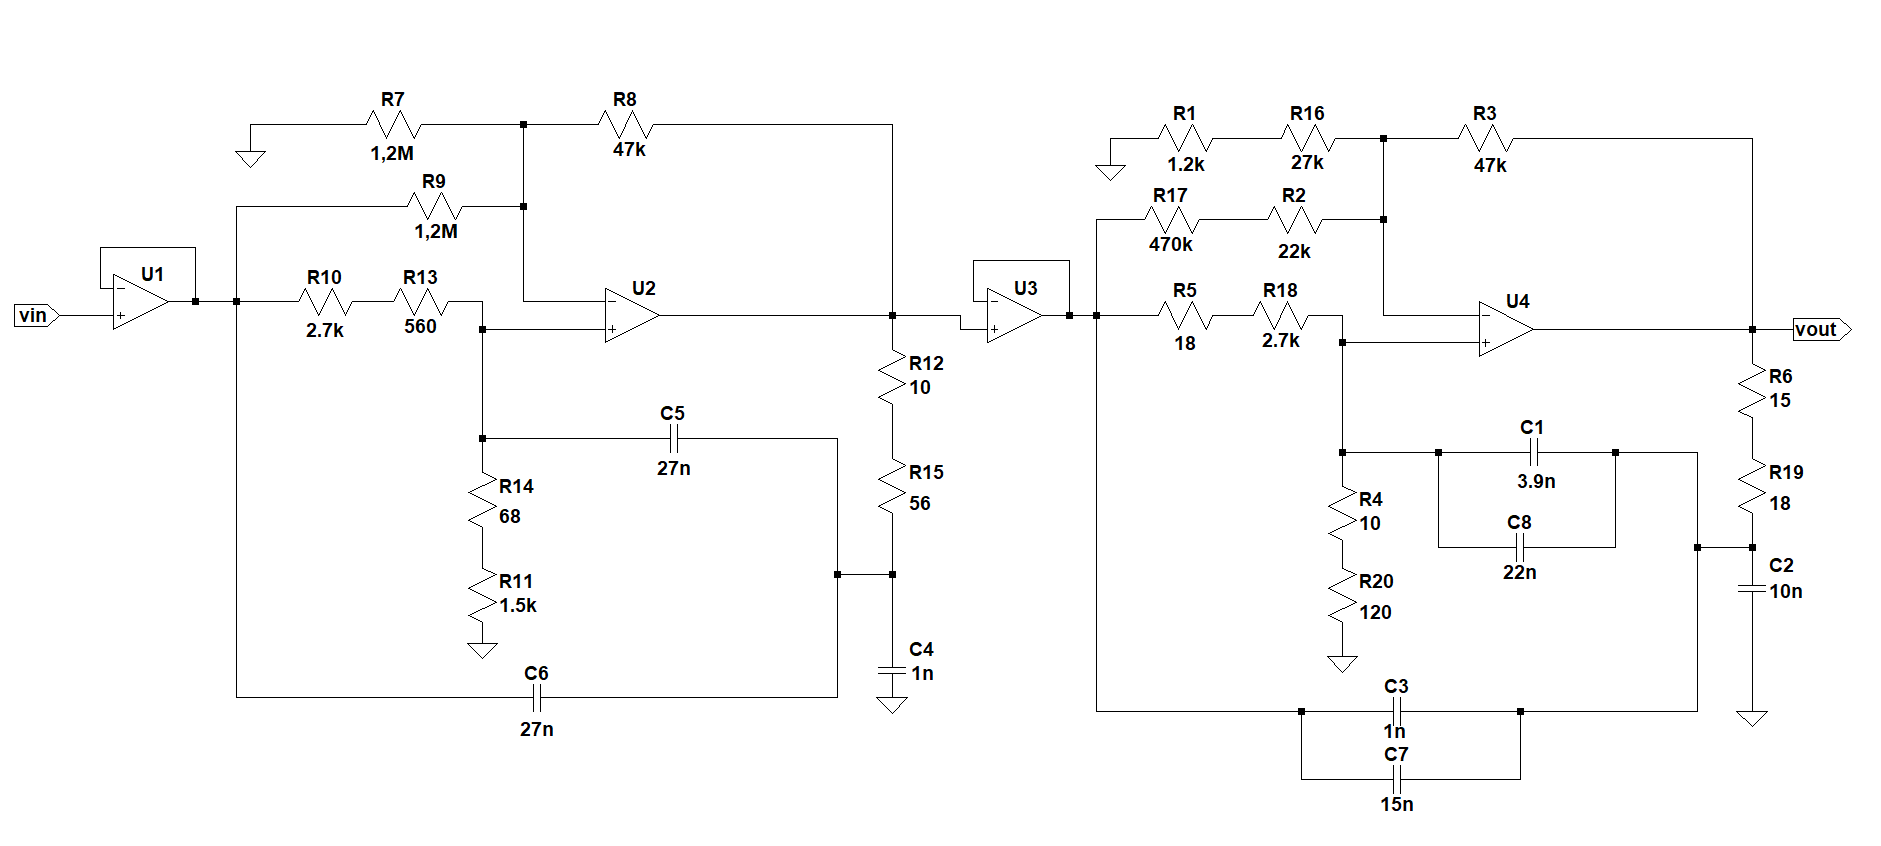
\includegraphics[width=0.9\textwidth]{../EJ3/Resources/filter_buffered.png}
    \caption{Circuito del filtro con buffers}
     \label{EJ3_FILTER_CIRCUIT_BUFFERED}
\end{figure}

Implementado este circuito en PCB, se midi\'o la impedancia de entrada colocando un resistor de $100k\Omega$ en serie a la entrada del filtro. Los resultados se observan abajo.

\begin{figure}[H]
    \centering
    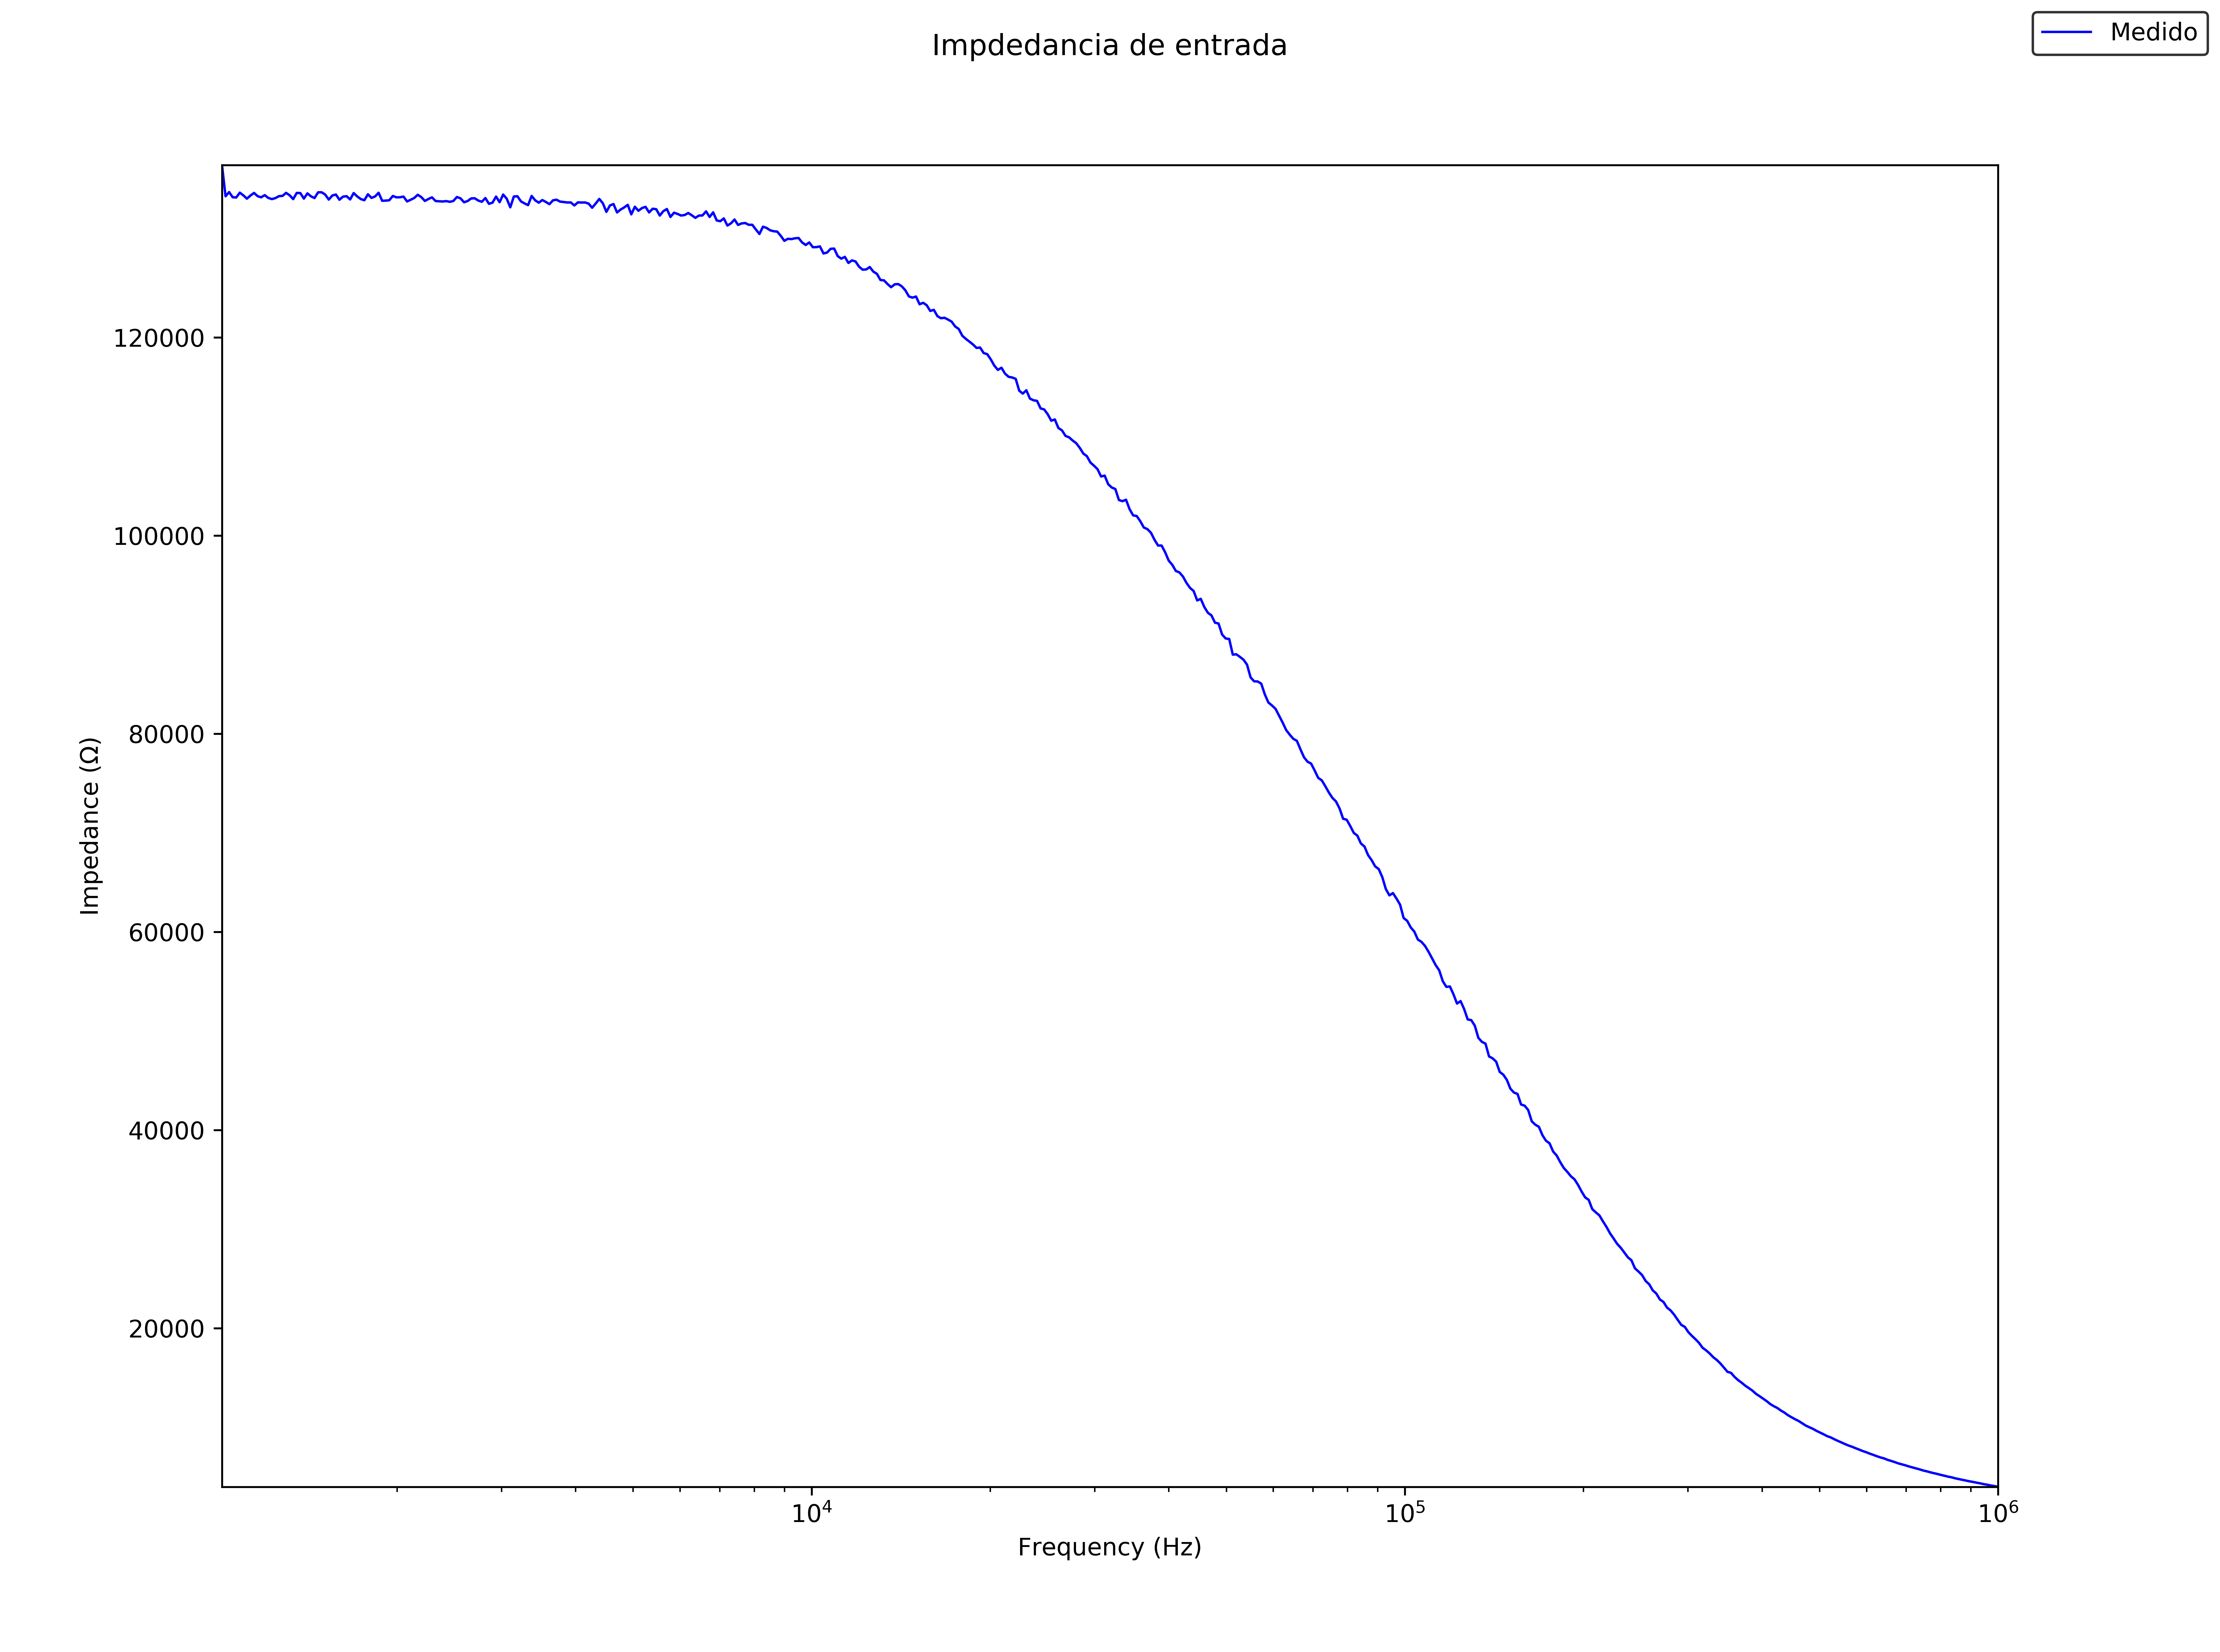
\includegraphics[width=0.9\textwidth]{../EJ3/Resources/zin_medida.png}
    \caption{Impedancia de entrada del filtro (medida)}
     \label{EJ3_ZIN_MEASURED}
\end{figure}

Respecto de la medici\'on se puede advertir que no coincide en orden de magnitud respecto de la simulaci\'on realizada en LTSpice. De todas formas, la impedancia de entrada se mantiene por encima de $50k\Omega$ hasta una frecuencia del orden de los $100kHz$, por lo que se considera satisfecho el requerimiento en este sentido.

\subsection{Ensayo de Montecarlo}

Antes de implementar el circuito en PCB se realiz\'o una verificaci\'on del dise\~no mediante un ensayo Montecarlo. Se asignaron las mismas tolerancias fijadas en la simulaci\'on de impedancia de entrada, y se obtuvo el siguiente resultado. Se superpone de forma aproximada la plantilla del filtro pedida.


\begin{figure}[H]
    \centering
    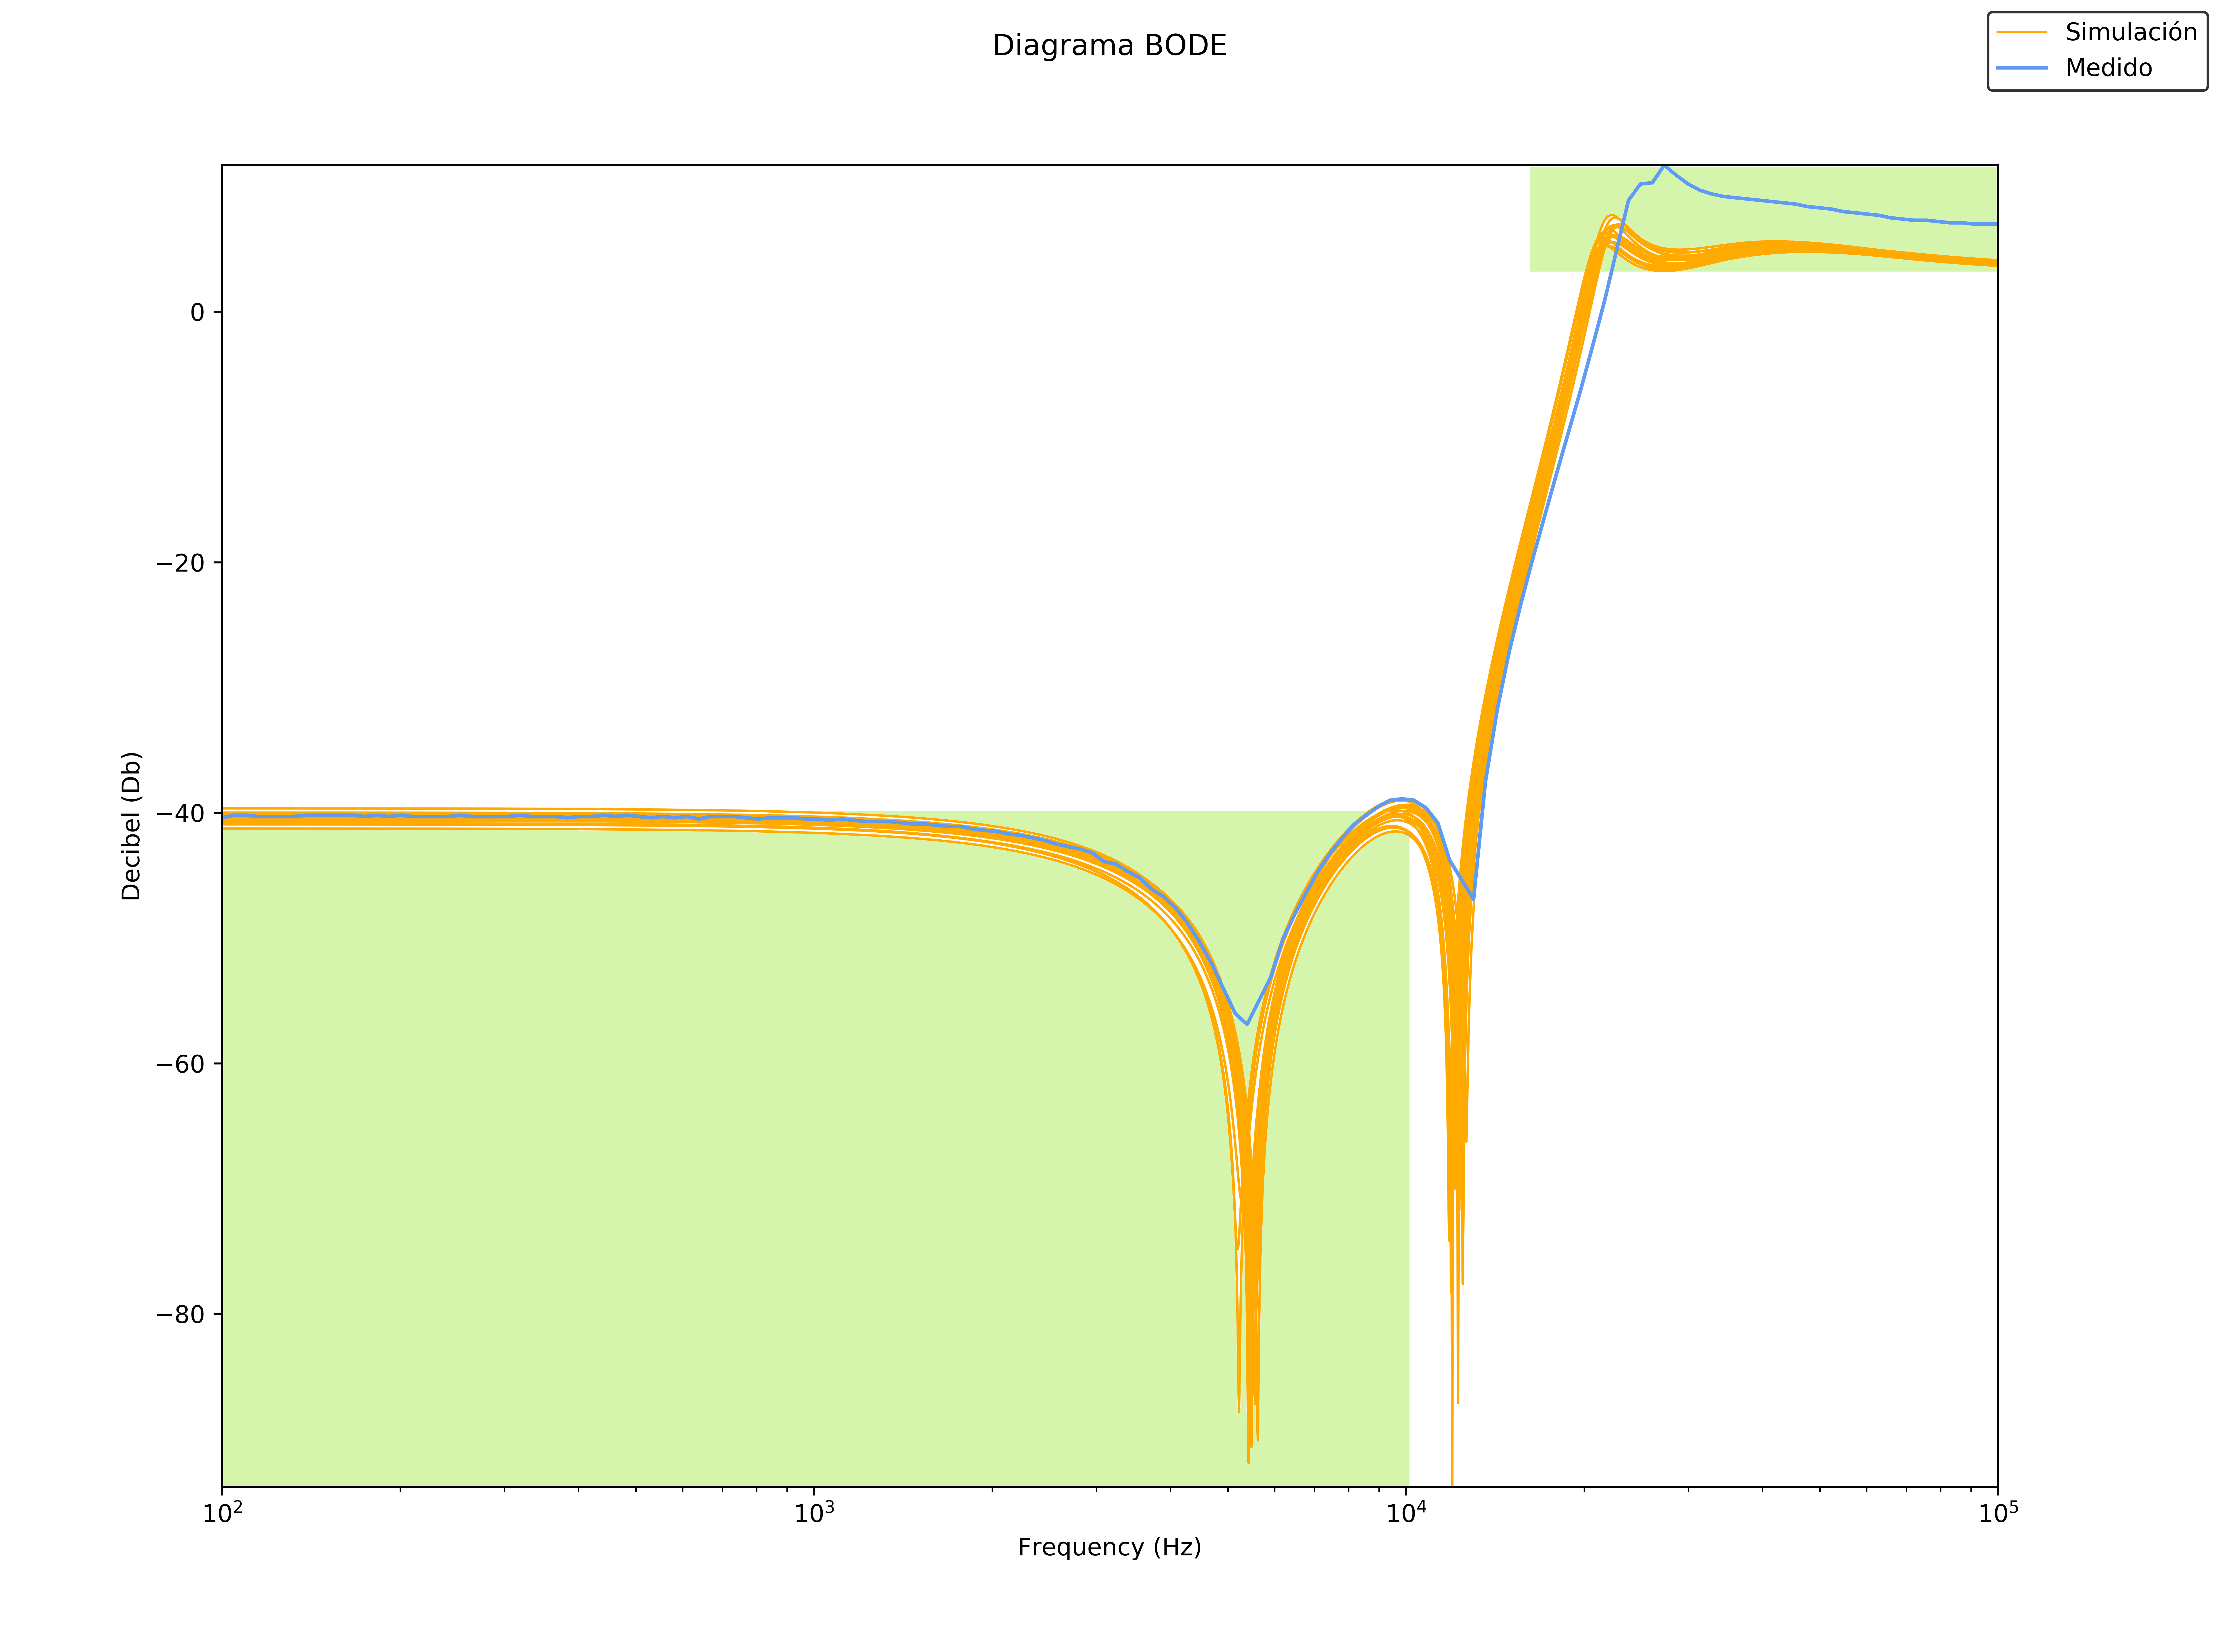
\includegraphics[width=0.9\textwidth]{../EJ3/Resources/montecarlo_plantilla2.png}
    \caption{Simulaci\'on Montecarlo del filtro - M\'odulo}
     \label{EJ3_FILTER_MONTECARLO}
\end{figure}

Respecto de esto, se puede advertir que em l\'ineas genereales el filtro cumple con las especificaciones de plantilla (resaltada en color verde). Se observa una peque\~na anormalidad entre los dos picos de atenuaci\'on, pero no se considera de tal relevancia como para invalidar el dise\~no. Adem\'as, el gr\'afico correspondiente al circuito real se encuentra por fuera del diagrama que comprende las tolerancias en los componentes.

Por otro lado, se realiza lo propio con la fase del circuito.

\begin{figure}[H]
    \centering
    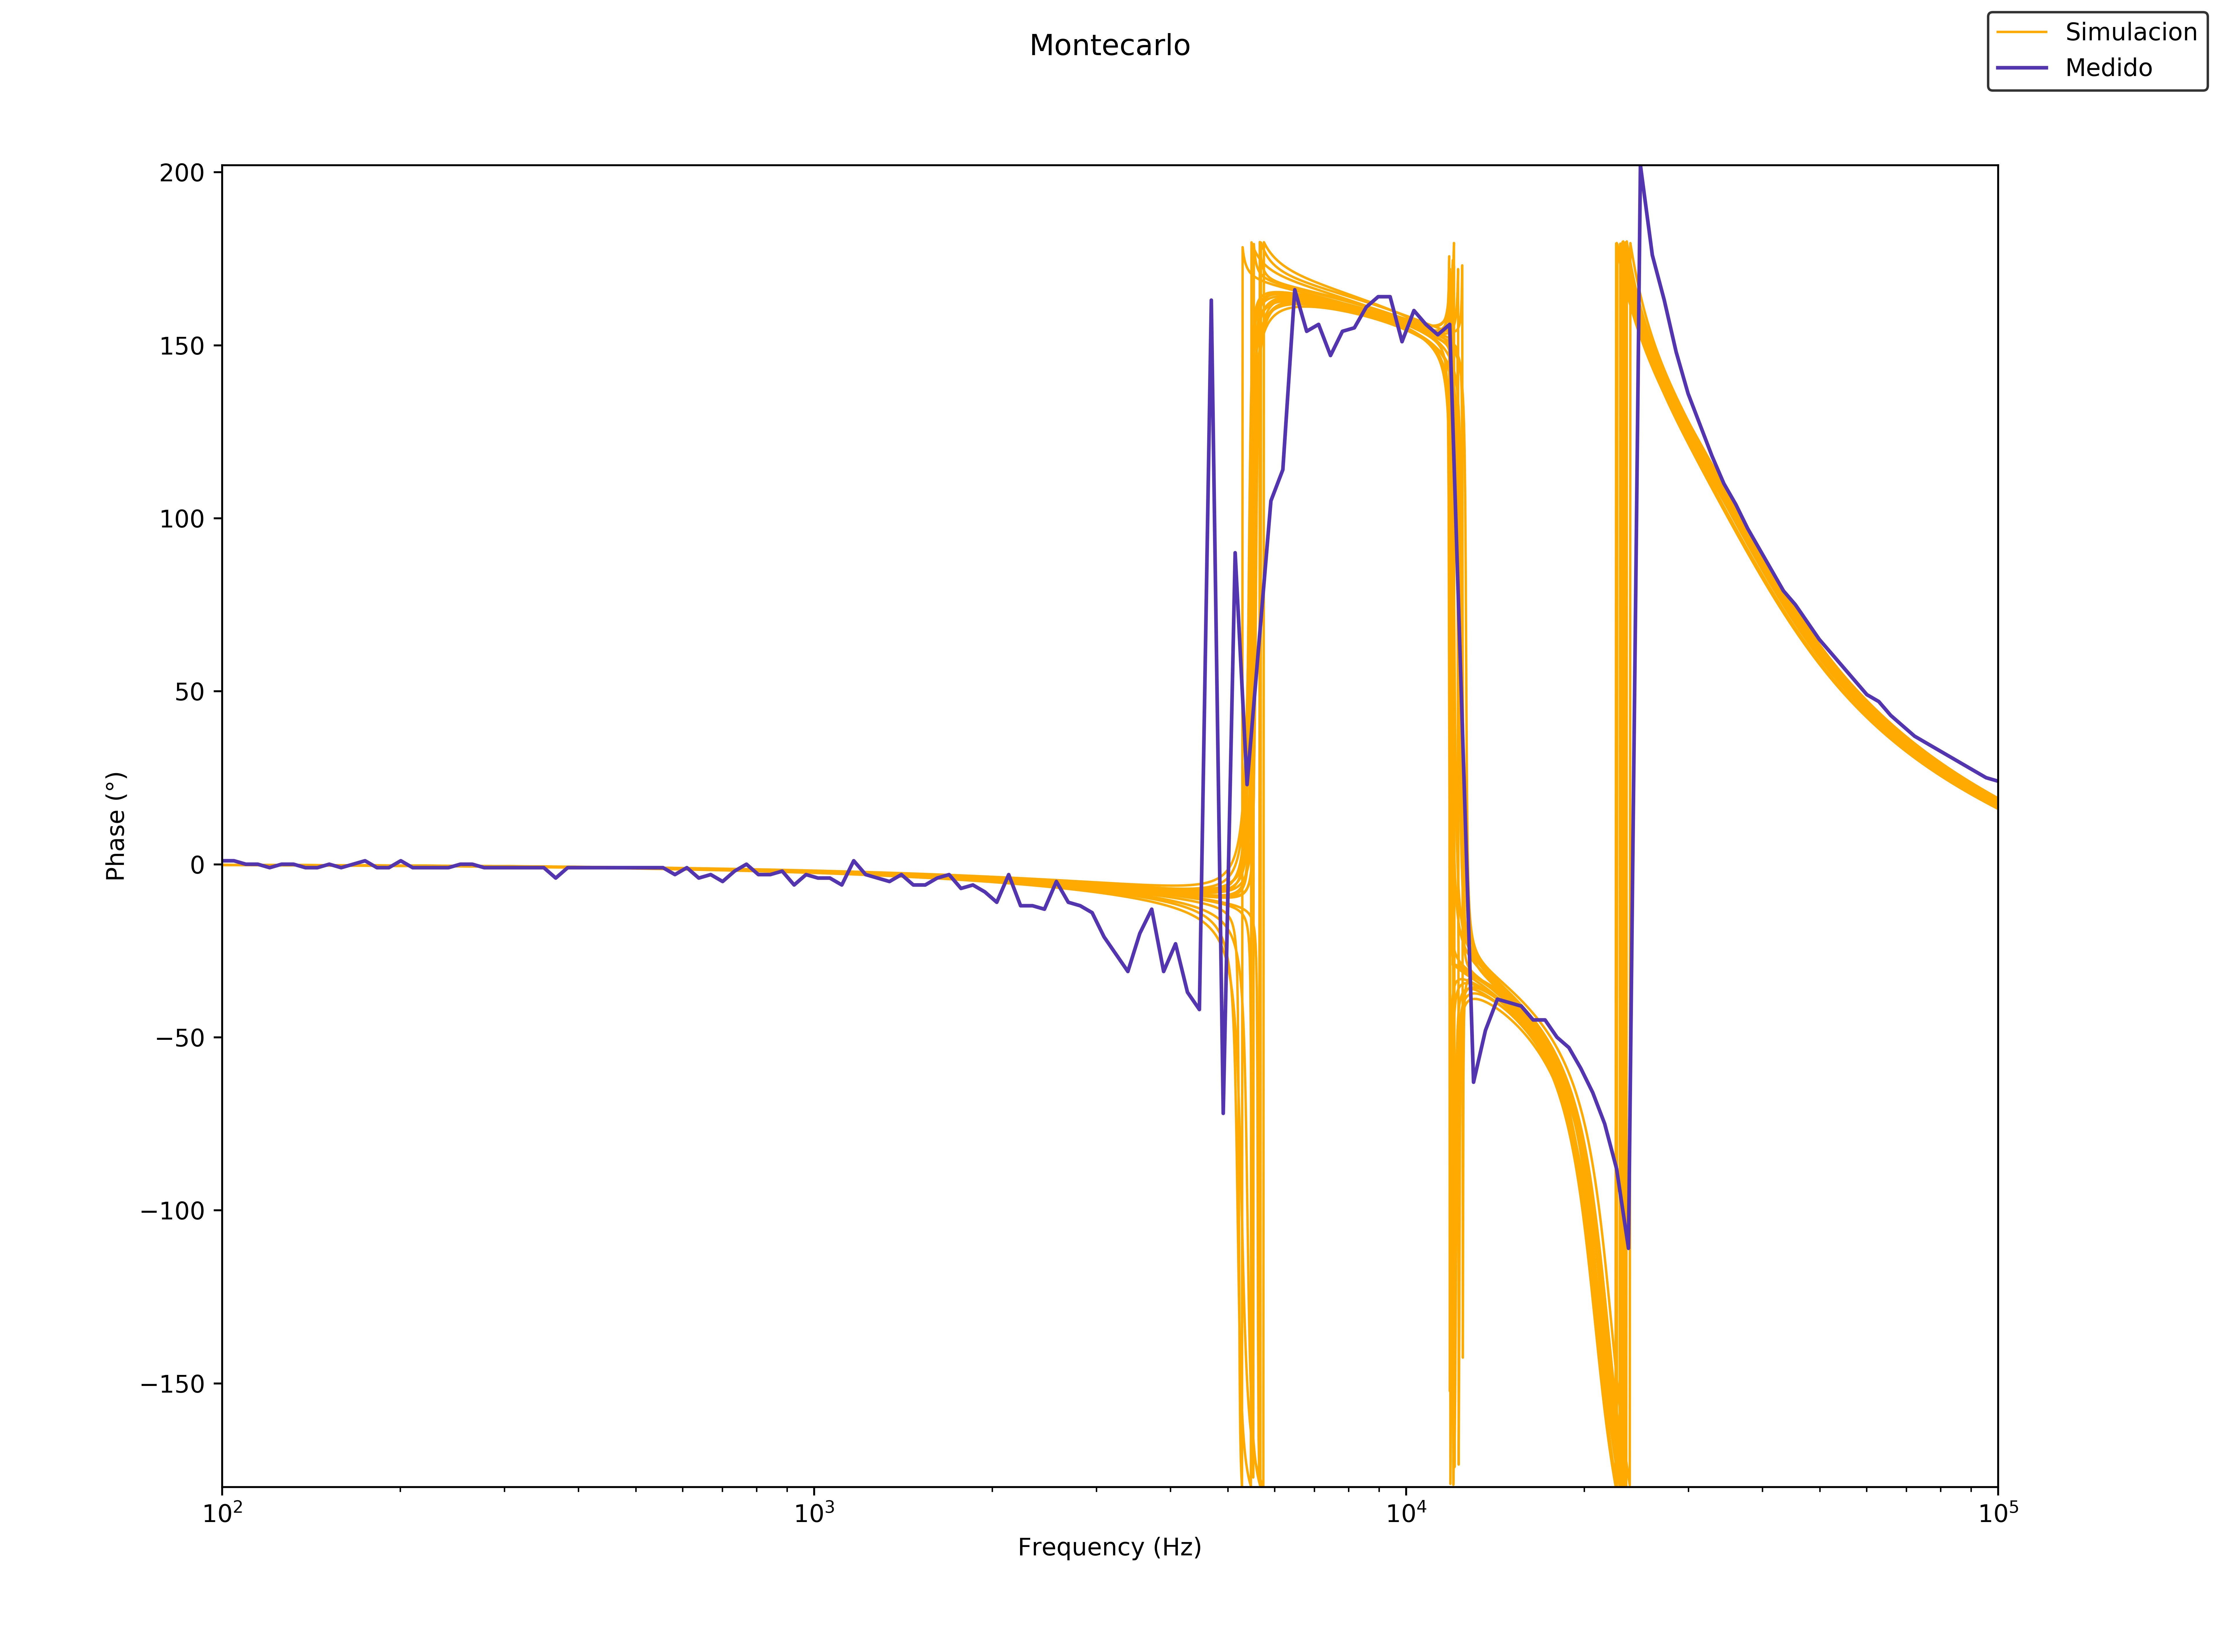
\includegraphics[width=0.9\textwidth]{../EJ3/Resources/montecarlo_phase.png}
    \caption{Simulaci\'on Montecarlo del filtro - Fase}
     \label{EJ3_FILTER_MONTECARLO_PHASE}
\end{figure}

\subsection{Rango din\'amico}

El rango din\'amico est\\a definido como la relaci\'on entre el piso de ruido y la tensi\\'on m\'axima que puede discernir el circuito.

\begin{equation}
\label{EJ3_RD}
RD = 20 \cdot log \left( \frac{V_i^{max}}{V_i^{min}}\right)
\end{equation}

El valor de $V_i^{min}$ se refiere al piso de ruido que se considere. En este caso, se supone un piso de ruido de $20mV$.

Respecto a $V_i^{max}$ es necesario observar el punto de ganancia m\'axima del sistema en el gr\'afico~\ref{EJ3_FILTER_MONTECARLO}. Este corresponde a un valor de $11,7dB$ a una frecuencia de aproximadamente $27,3kHz$. Esta ganancia equvale a 1,8 veces. Luego,

\begin{equation}
V_i^{max} = \frac{13,5 V}{1,8} \approx 7,5 V
\end{equation}

Donde $13,5V$ es el m\'aximo valor de salida del amplificador operacional (en este caso, TL082) siendo alimentado con $\pm 15V$.


Reemplazando los valores en la ecuaci\'on~\ref{EJ3_RD} se llega a:

\begin{equation}
RD \approx 51,48dB
\end{equation}

\subsection{Conclusi\'on}

A modo de conclusi\'on se puede destacar que se ha logrado dise\~nar dos celdas SGM que cumplen con las especificaciones pedidas. Se observa que en una peque\~na zona de frecuencias el filtro no responde como lo esperado, teniendo en cuenta los m\'argenes de seguridad adoptados en las ganancias en banda atenuada y pasante. Probablemente esto sea atribu\'ible a la dispersi\'on en los  valores de los componentes, que van m\'as all\'a de las tolerancias informadas por el fabricante. Tambi\'en se hace \'enfasis en la claridad del paper \textit{Optimum configurations for Single-Amplifier Biquadratic Filters}, mas espec\'ificamente en el proceso de dise\~no de la celda en s\'i misma. Por \'ultimo, se destaca que no se emplearon presets en el PCB final, lo que habla de un dise\~no del circuito lo suficientemente estable como para no necesitarlo.